\documentclass[12pt,openany]{extbook}
% \documentclass[a4paper,17pt]{extarticle}
\usepackage[a4paper, total={7in, 10in}]{geometry}
\usepackage[utf8]{inputenc}
\DeclareUnicodeCharacter{2212}{-}
\DeclareUnicodeCharacter{2502}{|}
\DeclareUnicodeCharacter{200B}{ }
\usepackage[russian]{babel}
\usepackage{graphicx}
\usepackage{float}
\usepackage{stackengine}
\usepackage{multicol}
\usepackage{amsfonts}
\usepackage{hyperref}
\usepackage[margin=10pt,font=footnotesize,labelfont=bf,labelsep=endash]{caption}
\newenvironment{Figure}{\par\medskip\noindent\minipage{\linewidth}}{\endminipage\par\medskip}
\setlength{\headheight}{14.5pt}
\usepackage{titling}
\newcommand{\subtitle}[1]{%
  \posttitle{%
    \par\end{center}
    \begin{center}\large#1\end{center}
   }%
}
\renewcommand{\baselinestretch}{1.15} 


% Для химических формул
% \usepackage[version=4]{mhchem}

% Для матеши
\usepackage{amsmath}
\usepackage{amssymb}

\usepackage{fancyhdr}
\newcommand{\bosversion}{v1.0.\hbox{\today}}

\pagestyle{fancy}
\fancyhf{}
\rhead{\rightmark}
\lhead{\leftmark}
\makeatletter
\let\ps@plain\ps@fancy % plain style = fancy style
\makeatother
% \rfoot{Стр. \thepage}
\fancyfoot[LE,RO]{Стр. \thepage/49}
\fancyfoot[RE,LO]{\href{https://qazcho.kz}{qazcho.kz}}
% \fancyfoot[R]{\thepage} % except the right
% \renewcommand{\contentsname}{Hello}
% \addto\captionrussian{% Replace "english" with the language you use
%   \renewcommand{\contentsname}%
%     {Hello}%
% }
% \usepackage{helvet}

% \renewcommand{\sfdefault}{ptm}
% \usepackage{sectsty}
% \allsectionsfont{\sffamily\bfseries}
% \setlength{\beforechapskip}{20pt}
\makeatletter
\renewcommand{\@chapapp}{Раздел}
\makeatother

\usepackage[x11names]{xcolor}
\usepackage{framed}
\usepackage{quoting}

 \colorlet{shadecolor}{LavenderBlush2}
\usepackage{lipsum}
\newenvironment{shadedquotation}
 {\begin{shaded*}
  \quoting[leftmargin=0pt, vskip=0pt]
 }
 {\endquoting
 \end{shaded*}
}

\usepackage{xcolor}

\usepackage{lipsum} % for mock text

\newsavebox{\coloredquotationbox}
\newenvironment{coloredquotation}
 {%
  \begin{trivlist}
  \begin{lrbox}{\coloredquotationbox}
  \begin{minipage}{\dimexpr\linewidth-2\fboxsep}
 }
 {%
  \end{minipage}
  \end{lrbox}
  \item\relax
  \parbox{\linewidth}{
    \begingroup
    \color[RGB]{224,215,188}%
    \hrule
    \color[RGB]{249,245,233}%
    \hrule
    \color[RGB]{224,215,188}%
    \hrule
    \endgroup
    \colorbox[RGB]{249,245,233}{\usebox{\coloredquotationbox}}\par\nointerlineskip
    \begingroup
    \color[RGB]{224,215,188}%
    \hrule
    \color[RGB]{249,245,233}%
    \hrule
    \color[RGB]{224,215,188}%
    \hrule
    \endgroup
  }
  \end{trivlist}
 }

\usepackage{titlesec}

\titlespacing*{\section} {0pt}{2.5ex plus 1ex minus .2ex}{1.3ex plus .2ex}
\titlespacing*{\subsection} {0pt}{2.25ex plus 1ex minus .2ex}{0.5ex plus .2ex}

\begin{document}

\begin{titlepage}


\newcommand{\HRule}{\rule{\linewidth}{0.5mm}} % Defines a new command for the horizontal lines, change thickness here

\center % Center everything on the page


\includegraphics[width=0.5\linewidth]{logo_color.jpg}\\[1.0cm]

%----------------------------------------------------------------------------------------
%	HEADING SECTIONS
%----------------------------------------------------------------------------------------

\begin{minipage}{0.5\textwidth}
\begin{flushleft} \large
\textsc{\textbf{Республиканская Коллегия Составителей Задач по Олимпиадной Химии}}
\end{flushleft}
\end{minipage}
~
\begin{minipage}{0.4\textwidth}
\begin{flushright} \large
\textsc{\textbf{Профиль участника РО (2022-2023 уч. год)}}\\
\textsc{\today}
\end{flushright}
\end{minipage}\\[2.0cm]

\begin{minipage}{0.93\textwidth}
\begin{flushleft}
  

\textbf{\large Введение}\\[0.5cm]
В 2022-2023 уч. году, комплекты заданий районного, областного и заключительного этапов республиканской олимпиады школьников по химии (далее - РО) сопровождались призывом к участникам оставить обратную связь по прошедшей олимпиаде путем заполнения онлайн опроса, созданного Республиканской Коллегией Составителей Задач по Олимпиадной Химии (далее - Коллегия). 
\vspace{0.5em}

Первостепенной задачей опроса было получение информации о том, как ученики готовятся к олимпиадам и насколько сложными, объемными и интересными им показались задания. Дополнительно была собрана демографическая информация. В этой заметке предоставляем результат анализа собранных ответов. В дополнении, анализируем результаты областного и заключительного этапов РО-2023, сравниваем их с результатами предыдущих годов.
\vspace{0.5em}

Главная задача при написании этого документа - улучшить представления составителей заданий о том, какой уровень подготовки имеется у участников того или иного этапа РО. 
\vspace{0.5em}

Код, с помощью которого был произведен анализ данных, доступен на \href{https://github.com/anmorgunov/respa-data-analysis}{Github}. Там же есть все графики, которые есть в этом документе. Если вы предпочитаете самостоятельно изучать информацию - приглашаю вас \href{https://github.com/anmorgunov/respa-data-analysis/tree/main/export/pdf}{в папку /export/pdf/}.
\end{flushleft}
\end{minipage}


\end{titlepage}


\def\contentsname{Содержание}
\tableofcontents

% \section{Введение}

Когда в начале 2019 года меня пригласили быть руководителем сборной РК по химии, я с удивлением обнаружил, что несмотря на то, что республиканская олимпиада школьников по химии (и связанные с ней мероприятия) проходит уже почти 30 лет, у руководителей сборной нет никаких данных, на которые можно было бы опираться при принятии решений. Мы не могли ответить на элементарные вопросы: насколько хорошо ученики справлялись с похожими заданиями в предыдущие годы? Насколько хорошо они пишут районную олимпиаду? А областную? Насколько хорошо областная олимпиада готовит учеников к заключительному этапу? А кто участвует на каждом этапе? Какое распределение по школам? Как много учеников неспециализированных школ? Насколько осведомлены участники разных этапов о доступных для них ресурсах?

Хочется верить, что за почти 5 лет вовлеченности в олимпийское движение, я смог хоть немного, но уменьшить долю хаоса и увеличить количество структурированной информации. Текущий документ - попытка свести собранную информацию об участниках РО в единый документ, в надежде, что последующие руководители сборных смогут пользоваться им для принятия \textit{data-driven decisions}. 

Код, с помощью которого был произведен анализ данных, доступен на \href{https://github.com/anmorgunov/respa-data-analysis}{Github}. Там же есть все графики, которые есть в этом документе. Если вы предпочитаете самостоятельно изучать информацию - приглашаю вас \href{https://github.com/anmorgunov/respa-data-analysis/tree/main/export/pdf}{в папку /export/pdf/}.


\textit{\\
С уважением,\\
Моргунов Антон\\
Председатель Коллегии и руководитель сборной (2019-2023)}

% \chapter{Подготовка заданий}
% Поскольку решения, о которых пойдет речь в этой секции, в основном принимались председателем Коллегии (Моргунов А.), текст этого раздела написан от имени председателя Коллегии.

\section{Уроки предыдущего учебного года}

Концептуальные решения о том, какими будут задания районного, областного и заключительного этапа РО в этом году принимались под влиянием уроков и выводов, сделанных по результатам предыдущего цикла РО (см. \href{https://qazcho.kz/docs/reports/qazcho_respa_analysis.pdf}{Аналитическую записку по результатам РО-2022} и \href{https://qazcho.kz/docs/reports/2021-2022-report.pdf}{Отчет о работе Коллегии QazChO за 2021-2022 академический год}). 

\subsection{Сложность олимпиад}

В прошлом году было констатировано снижение уровня подготовки школьников (например, далко не все участники заключительного этапа справлялись с заданиями школьной программы). Поэтому, на ежегодном общем заседании Коллегии (\href{https://qazcho.kz/docs/public-protocols/protocol10.pdf}{Протокол №10 от 27 августа 2022}) было принято решение ввести разделение на «задачи с коротким условием» и «задачи с длинным условием» и принять некоторые правила о градации количества «задач, с коротким условием» по мере продвижения по этапам РО и классам участия. Осознанный фокус на создание определенного количества задач с коротким условием позволил значительно упростить сложность районного и областного этапов РО, изменение, которое было положительно оценено подавляющим большинством участников (см. Раздел 3. Восприятие олимпиады). На заключительном этапе в 10-11 классах была всего одна задача с коротким условием, что, возможно, отразилось на сложности комплекта - ученики посчитали, что заключительный этап был сложнее, чем в предыдущие годы. 

В дополнении, в этом учебном году, впервые в истории, все задания всех этапов РО оценивались на объем и сложность бывшими олимпиадниками, которые решали эти задания на время. Внедрение апробации позволило значительно сократить количество опечаток и ошибок в условиях, но, к сожалению, не привело к их полному исчезновению. В этом году задания решал только один олимпиадник (Касымалы Мадияр, золотой медалист IChO 2022); вполне возможно, что к апробации нужно привлекать больше одного человека. Примечательно, что несмотря на то, что Касымалы М. считал, что комплект заданий заключительного этапа сложнее, чем в предыдущие годы, он был крайне удивлен результатам учащихся: они были ниже, чем он ожидал. Тоже самое можно сказать и про остальных членов Коллегии: мы понимали, что задания немного сложнее, но не ожидали таких низких результатов (см. комментарии по задачам в разделе Результаты РО.) Вероятно, что к апробации стоит привлекать олимпиадников с варьирующимся уровнем подготовки, дабы лучше оценивать сложность олимпиады.

\subsection{Устойчивость процесса составления}

Предыдущий цикл РО можно назвать «травмирующим». К некоторым этапам, некоторые составители готовили по 3-5 задач. С одной стороны, небольшое количество составителей приводило к более сбалансированным и органичным комплектам заданий: во-первых, один и тот же составитель не будет делать две похожие задачи, во-вторых, коммуникация с меньшим количеством участников происходит быстрее и эффективнее. К сожалению, такой подход не является устойчивым в долгосрочной перспективе. После заключительного этапа РО-2022, я боялся, что мы можем потерять чуть ли не половину составителей, которые не захотят продолжать делать задания в последующие годы. Ситуация усугублялась хамскими, враждебными и пренебрежительными действиями РНПЦ Дарын (см. \href{https://qazcho.kz/docs/reports/qazcho_respa_analysis.pdf}{Аналитическую записку по результатам РО-2022}), которые приводили к полной потере желания что-либо делать. Учитывая такую обстановку, в этом году я принял решение постараться максимально снизить количество задач, которое составляет один автор, а также максимизировать свободу в действиях минимизируя количество требований и правок (я действовал из допущения, что учитывая то, что работа по составлению задач не является высокооплачиваемой, авторы могут получать моральное удовлетворение за счет возможности делать то, что хотят в первую очередь они сами). В результате, в Коллегию были привлечены 3 новых составителя, а составлением заданий РО занимались рекордные 14 человек (над одним заключительным этапом трудились, тоже рекордные, 12 человек).

\textbf{Составители заданий в цикле РО 2022-2023:}\vspace{-1em}
\begin{align*}
    &\text{Аманжолов Азим} & &\text{Жаксылыков Азамат} & &\text{Курамшин Болат} & &\text{Молдагулов Галымжан} \\
    &\text{Бегдаир Санжар} & &\text{Загрибельный Богдан} & &\text{Мадиева Малена} & &\text{Мужубаев Абильмансур} \\
    &\text{Бекхожин Жанибек} & &\text{Касьянов Артем} & &\text{Мельниченко Даниил} & &\text{Тайшыбай Айдын} \\
    &\text{Галикберова Милана} & &\text{Моргунов Антон} & &\text{} & &\text{} 
\end{align*}

В результате, один составитель предлагал не больше 2-3 задач, что значительно повысило устойчивость процесса подготовки комплектов заданий. Следующая задача - прийти к тому, чтобы количество предлагаемых задач на каждый этап превышало количество требуемых задач, дабы была возможность выбирать и создавать более органичный комплект. Для выполнения этой задачи необходимо и дальше привлекать новых составителей в Коллегию.

\subsection{Внедрение \LaTeX}

Традиционно, после получения всех задач, председатель Коллегии тратил 2-3 рабочих дня на компоновку заданий в единый комплект, что подразумевает приведение к общему формату, исправление маленьких ошибок, правильная нумерация, правильные и одинаковые отступы и так далее. Для минимизации времени, которое уходит на визуальное оформление комплекта заданий было принято решение перейти на оформление заданий в \LaTeX. Новый член Коллегии Жаксылыков А. разработал невероятно красивый и удобный шаблон (\href{https://github.com/Beyond-Curriculum/qazcho-latex}{доступный на Github}), который позволил свести на нуль время, необходимое на оформление заданий.


\section{Задания районного этапа}
Подготовка заданий началась 5 сентября 2022 г. Составителям был поставлен дедлайн 23 октября. Одновременно поставлены дедлайны для заданий областного (27 ноября) и заключительного (26 февраля) этапов. Было предложено следующее распределение по кол-ву задач с коротким и длинным условием:

\begin{table}[h]
    \centering
    \begin{tabular}{|c|c|c|}
        \hline
        Класс & Кол-во задач с коротким условием & Кол-во задач с длинным условием \\ \hline
        9 & 3 & 1 \\ \hline
        10 & 3 & 2 \\ \hline
        11 & 3 & 2 \\ \hline
    \end{tabular}
    \label{tab:tasks}
\end{table}

По темам составителям была предоставлена полная свобода. Единственное, что было принято решение не составлять задания по органической химии в 9 и 10 класс. В рамках \href{https://qazcho.kz/docs/npa/respa-syllabus.pdf}{Концепции тем и сложности РО (далее - силлабус)}, систематические знания органической химии ожидаются с областного этапа 10 кл. На всех этапах 9 кл. и районном этапе 10 кл. подразумевалось знание \textit{школьной органики}. Изначально, это понятие попало в силлабус поскольку в 9 кл. (особенно на заключительном этапе) традиционно были задачи по органике, но требовать системного понимания органики (например того, которое образуется после прочтения учебника \textit{John McMurry. Organic Chemistry}) раньше областного этапа 10 кл. было бы неразумным. На основании опыта предыдущих лет, к началу текущего цикла РО сформировалось четкое понимание, что задачи по \textit{школьной органике} крайне ограничены в своем разнообразии и в какой-то степени сильно типичны. Иными словами, либо каждый год Коллегия будет составлять примерно одни и те же задачи, либо так или иначе придется выходить за рамки \textit{школьной органики}. Это понимание подкреплялось наблюдением за некоторыми учениками 9 класса на \href{https://ask.bc-pf.org}{форуме Спроси}, которые начинали изучение учебников, предназначенных для учеников 10-11 классов.

\section{Задания областного этапа}
Подготовка заданий началась 18 ноября 2022 г. Было предложено следующее распределение по кол-ву задач с коротким и длинным условием:

\begin{table}[h]
    \centering
    \begin{tabular}{|c|c|c|}
        \hline
        Класс & Кол-во задач с коротким условием & Кол-во задач с длинным условием \\ \hline
        9 & 3 & 2 \\ \hline
        10 & 3 & 3 \\ \hline
        11 & 2 & 4 \\ \hline
    \end{tabular}
    \label{tab:tasks11}
\end{table}

Руководствуясь той же аргументацией, что и при подготовке заданий районного этапа, было решено не включать задания по органическому синтезу в 9 класс. Использование органических молекул и реакций в задачах на смеси и неизвестные вещества приветствовалось. 

При подготовке заданий областного этапа началось обсуждение концепции заключительного этапа, дабы задания области начинали готовить участников к заключительному этапу. Было предложено в этом году сделать фокус на т.н. научной грамотности (\textit{scientific literacy}): умение читать (интерпретировать)  графики, схемы, экспериментальные установки и т. д. В идеале, сделать что-то похожее на третью задачу IChO 2022 (основная сложность задачи сводилась к правильной интерпретации экспериментальной установки, сами расчеты были простыми), ибо такие задачи вызывают сложности у сборной РК. В результате, в комплекте заданий появился \textit{Органический блиц} (\href{https://olympiads.bc-pf.org/chemistry/oblast/2023/10}{Задача №10-5}) и \textit{Электрохимия возвращается} (\href{https://olympiads.bc-pf.org/chemistry/oblast/2023/11}{Задача №11-5}). 

\section{Задания заключительного этапа}

Подготовка заданий началась 23 января 2023 г. Было предложено следующее распределение по кол-ву задач с коротким и длинным условием:

\begin{table}[h]
    \centering
    \begin{tabular}{|c|c|c|}
        \hline
        Класс & Кол-во задач с коротким условием & Кол-во задач с длинным условием \\ \hline
        9 & 4 & 3 \\ \hline
        10 & 3 & 4 \\ \hline
        11 & 3 & 4 \\ \hline
    \end{tabular}
\end{table}

Руководствуясь той же аргументацией, что и на предыдущих этапах, было принято решение не делать задачу на органический синтез в 9 кл. Отдельно была сделана просьба делать 1-2 простых пункта/вопроса в каждой задаче.

Среди заданий, которые были предложены составителями к концу февраля, было недостаточно заданий с коротким условием. Более того, ряд заданий значительно отошли от изначальной задумки. К сожалению, на тот момент уже не оставалось времени (одна неделя выделялась на оформление, вычитку заданий и исправление ошибок, одна неделя на перевод) на значительные правки или составление новых задач, поэтому комплект был составлен из того, что было предложено. Скорее всего, в последующие годы рационально будет ставить дедлайн составления заданий заключительного этапа за два месяца до олимпиады, дабы было время заменить/значительно видоизменить предложенные задачи.

\chapter{Демографический профиль}
\section{Введение}

В 2022-2023 учебном году, комплекты заданий и решений теоретических туров районного, областного и заключительного этапов республиканской олимпиады школьников по химии сопровождались призывом оставить обратную связь о прошедшей олимпиаде, заполнив онлайн опрос, созданный Коллегией. Ссылка на опрос также дублировалась на официальных каналах Коллегии и на (\href{https://ask.bc-pf.org}{форуме Спроси}). В распространении опроса РНПЦ Дарын и Министерство Просвещения РК не принимали никакого участия. В рамках опроса, помимо «существенных» вопросов, ответы на которые проанализированы в других разделах, участники предоставляли демографические данные. Некоторые сводки настолько нас удивили, что мы решили посвятить им отдельную секцию.

Опрос по районному этапу РО прошли 40 участников. Из них 10 (25\%), 15 (37.5\%) и 15 (37.5\%) человек участвовали за 9, 10 и 11 класс соответственно. Распределение по школам следующее:

\begin{table}[ht]
    \centering
    \begin{tabular}{|l|c|c|}
    \hline
    \textbf{Тип школы} & \textbf{Количество} & \textbf{Процент} \\ \hline
    Обычная школа (в городе) & 16 & 40.0\% \\ \hline
    Обычная школа (в селе) & 12 & 30.0\% \\ \hline
    БИЛ & 8 & 20.0\% \\ \hline
    Другая специализированная школа & 2 & 5.0\% \\ \hline
    Частная школа & 2 & 5.0\% \\ \hline
    НИШ & 0 & 0.0\% \\ \hline
    РФМШ & 0 & 0.0\% \\ \hline
    \end{tabular}
    \caption{Типы школ и их распределение на районном этапе РО}
    \label{tab:region-schols}
\end{table}

Стоит заметить, что ученики НИШ и БИЛ не пишут районный этап и проходят сразу на областной, поэтому ответов от учеников НИШ нет. 8 ответов от учеников БИЛ скорее всего предоставлены учениками, которые самостоятельно прорешивали задания районного этапа.

Опрос по областному этапу РО прошли 60 участников. Из них 28 (46.7\%), 17 (28.3\%), и 15 (25.0\%) человек участвовали за 9, 10 и 11 класс соответственно. Распределение по школам следующее:

\begin{table}[ht]
    \centering
    \begin{tabular}{|l|c|c|}
        \hline
        \textbf{Тип школы} & \textbf{Количество} & \textbf{Процент} \\ \hline
        БИЛ & 31 & 51.7\% \\ \hline
        Другая специализированная школа & 11 & 18.3\% \\ \hline
        НИШ & 8 & 13.3\% \\ \hline
        Обычная школа (в городе) & 6 & 10.0\% \\ \hline
        Частная школа & 3 & 5.0\% \\ \hline
        РФМШ & 1 & 1.7\% \\ \hline
        Обычная школа (в селе) & 0 & 0.0\% \\ \hline
    \end{tabular}
    \caption{Типы школ и их распределение на областном этапе РО}
    \label{tab:obl-schools}
\end{table}

Нельзя не заметить практически полное отсутствие ответов от учников из неспециализированных школ. Конечно, 40 и 60 респондентов для этапа, на котором участвуют десятки тысяч (район) и тысячи (область) школьников, могут быть не репрезентативной выборкой. Однако, сложно представить, что ученики из неспециализированных школ, которые участвовали на районном этапе и заполняли опрос, не заполнили бы опрос на областном этапе, если бы они на нем участвовали. Таким образом, Таблица \ref{tab:obl-schools} может указывать на то, что ученики неспециализированных школ в своем большинстве не проходят дальше районного этапа.

Опрос по заключительному этапу РО прошли 32 участника. Из них 9 (28.1\%), 9 (28.1\%) и 14 (43.8\%) человек участвовали за 9, 10 и 11 класс соответственно. Распределение по школам следующее:

\begin{table}[ht]
    \centering
    \begin{tabular}{|l|c|c|}
    \hline
    \textbf{Тип школы} & \textbf{Количество} & \textbf{Процент} \\ \hline
    БИЛ & 15 & 46.9\% \\ \hline
    Другая специализированная школа & 5 & 15.6\% \\ \hline
    Обычная школа (в городе) & 5 & 15.6\% \\ \hline
    НИШ & 4 & 12.5\% \\ \hline
    Частная школа & 2 & 6.3\% \\ \hline
    РФМШ & 1 & 3.1\% \\ \hline
    Обычная школа (в селе) & 0 & 0.0\% \\ \hline
    \end{tabular}
    \caption{Типы школ и их распределение на заключительном этапе РО}
    \label{tab:respa-schools}
\end{table}

\section{Язык обучения и язык участия на РО}


\chapter{Восприятие олимпиады}
\section{Насколько задания были сложными?}

Участникам олимпиады, в рамках заполнения онлайн-опроса (см. Раздел 1 для получения профиля респондентов) было предложено оценить сложность олимпиады по 5-бальной шкале.

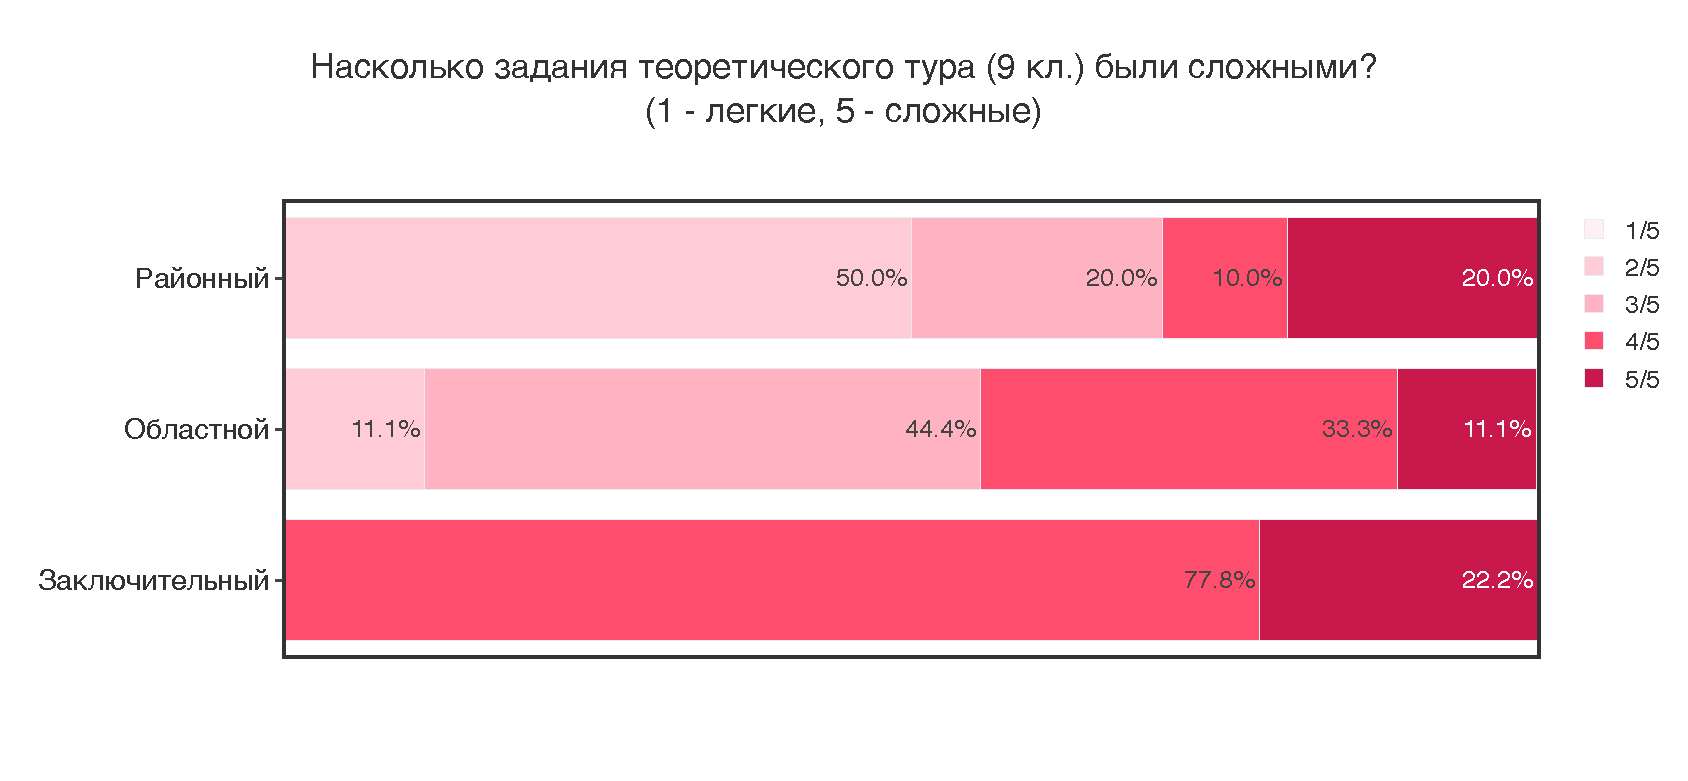
\includegraphics[width=\linewidth]{../export/pdf/demographics/difficulty-grade9.pdf}

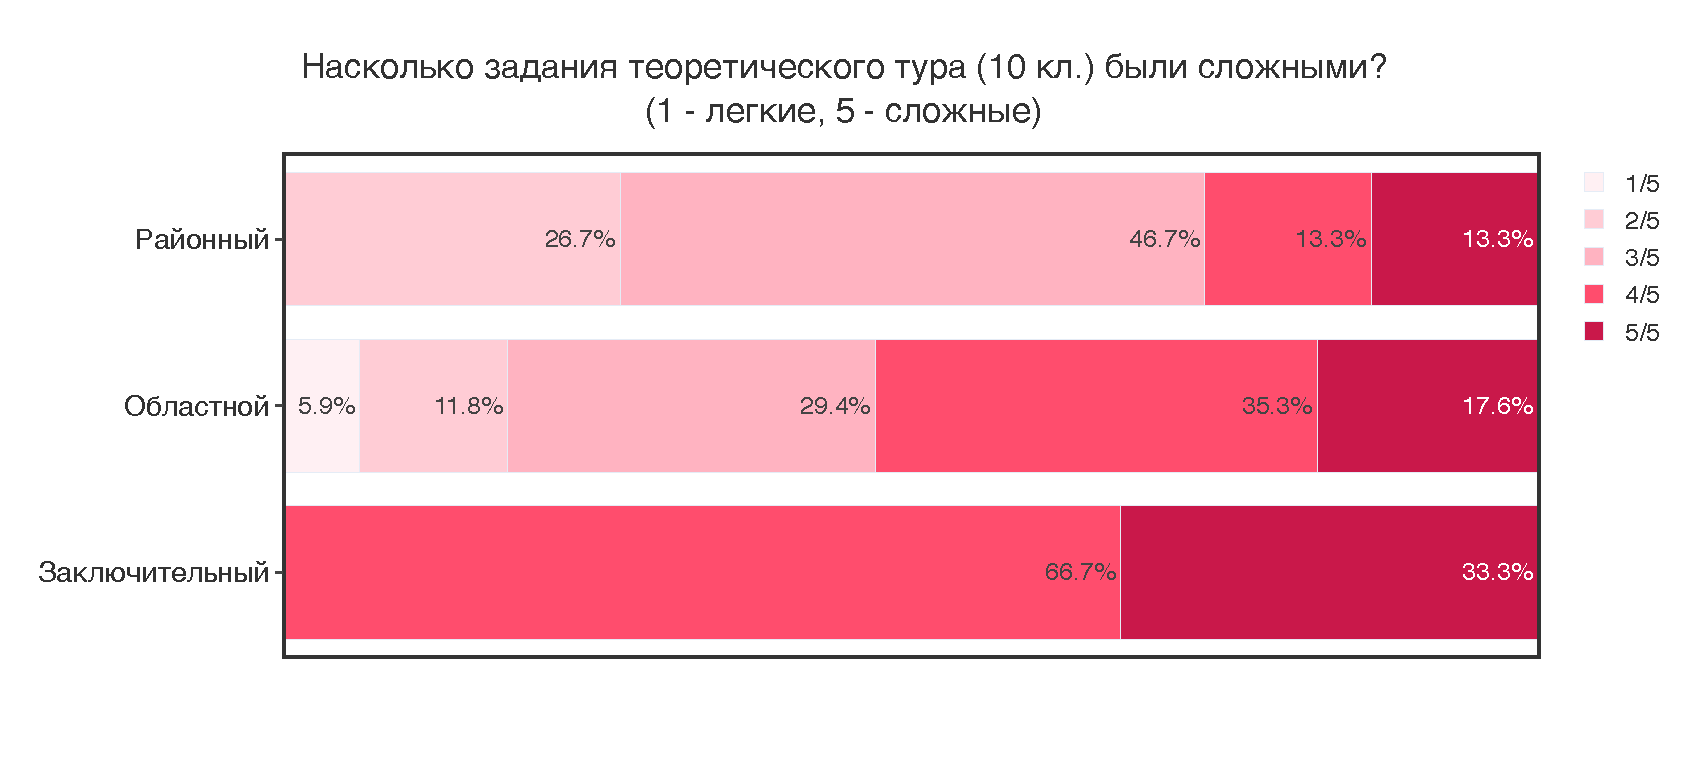
\includegraphics[width=\linewidth]{../export/pdf/demographics/difficulty-grade10.pdf}

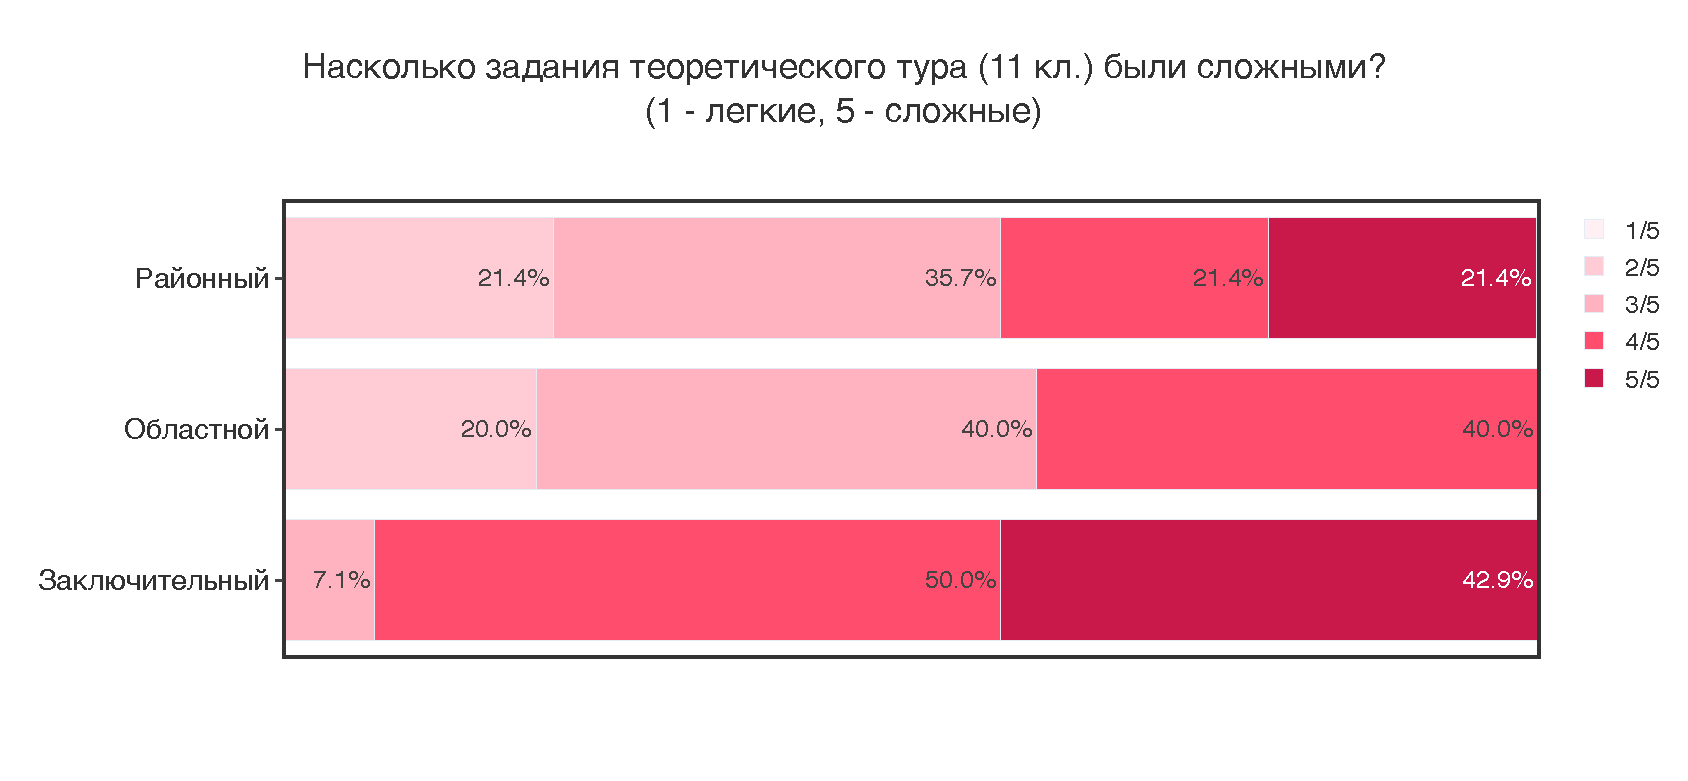
\includegraphics[width=\linewidth]{../export/pdf/demographics/difficulty-grade11.pdf}

\newpage
\section{Насколько задания были объемными?}

Участникам олимпиады предлагалось оценить насколько задания были объемными по 5-бальной шкале.

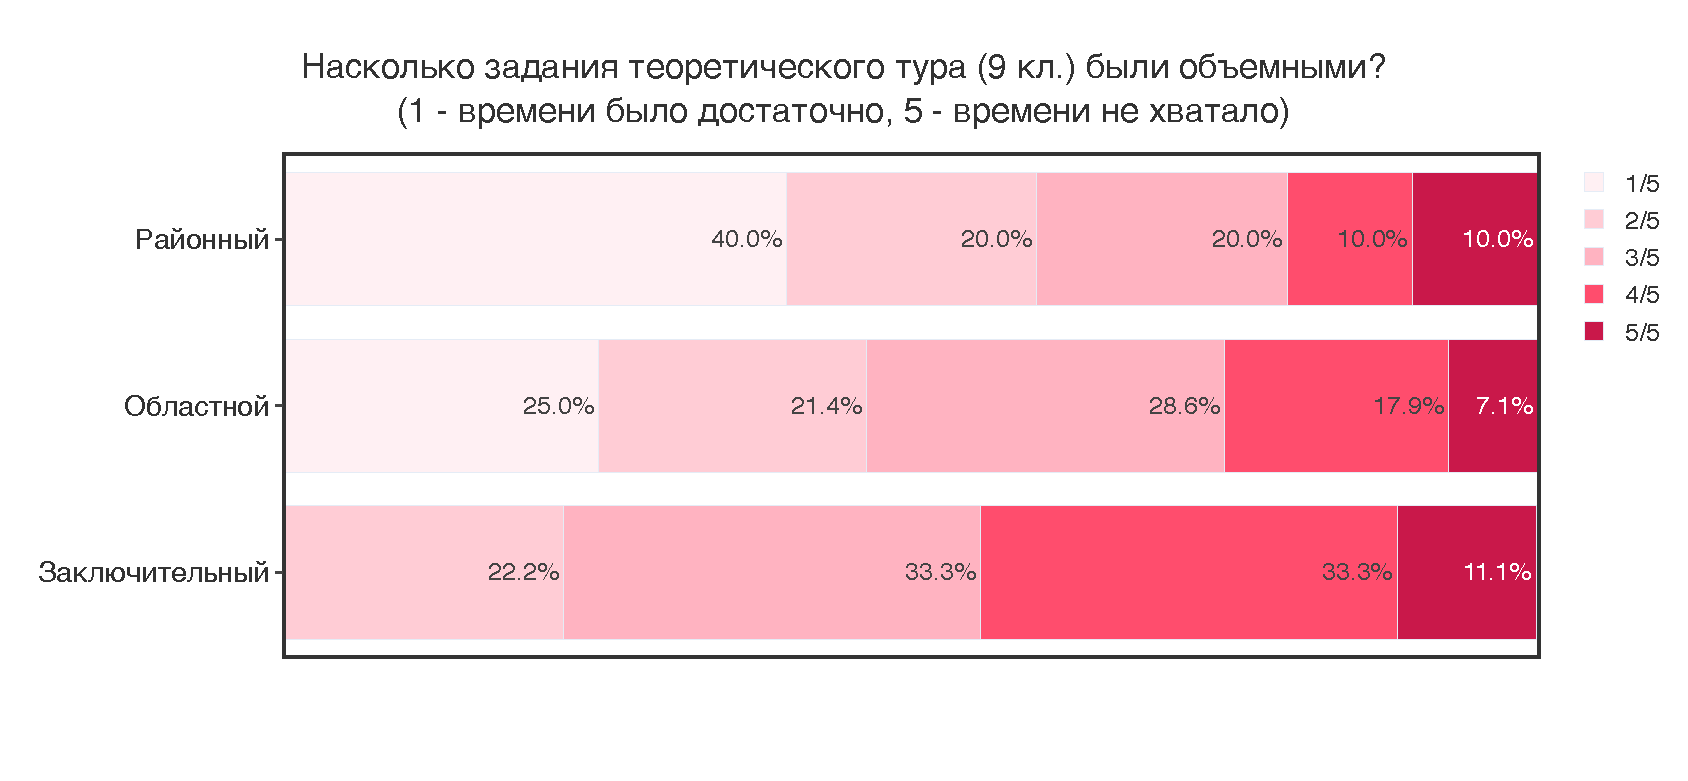
\includegraphics[width=\linewidth]{../export/pdf/demographics/volume-grade9.pdf}

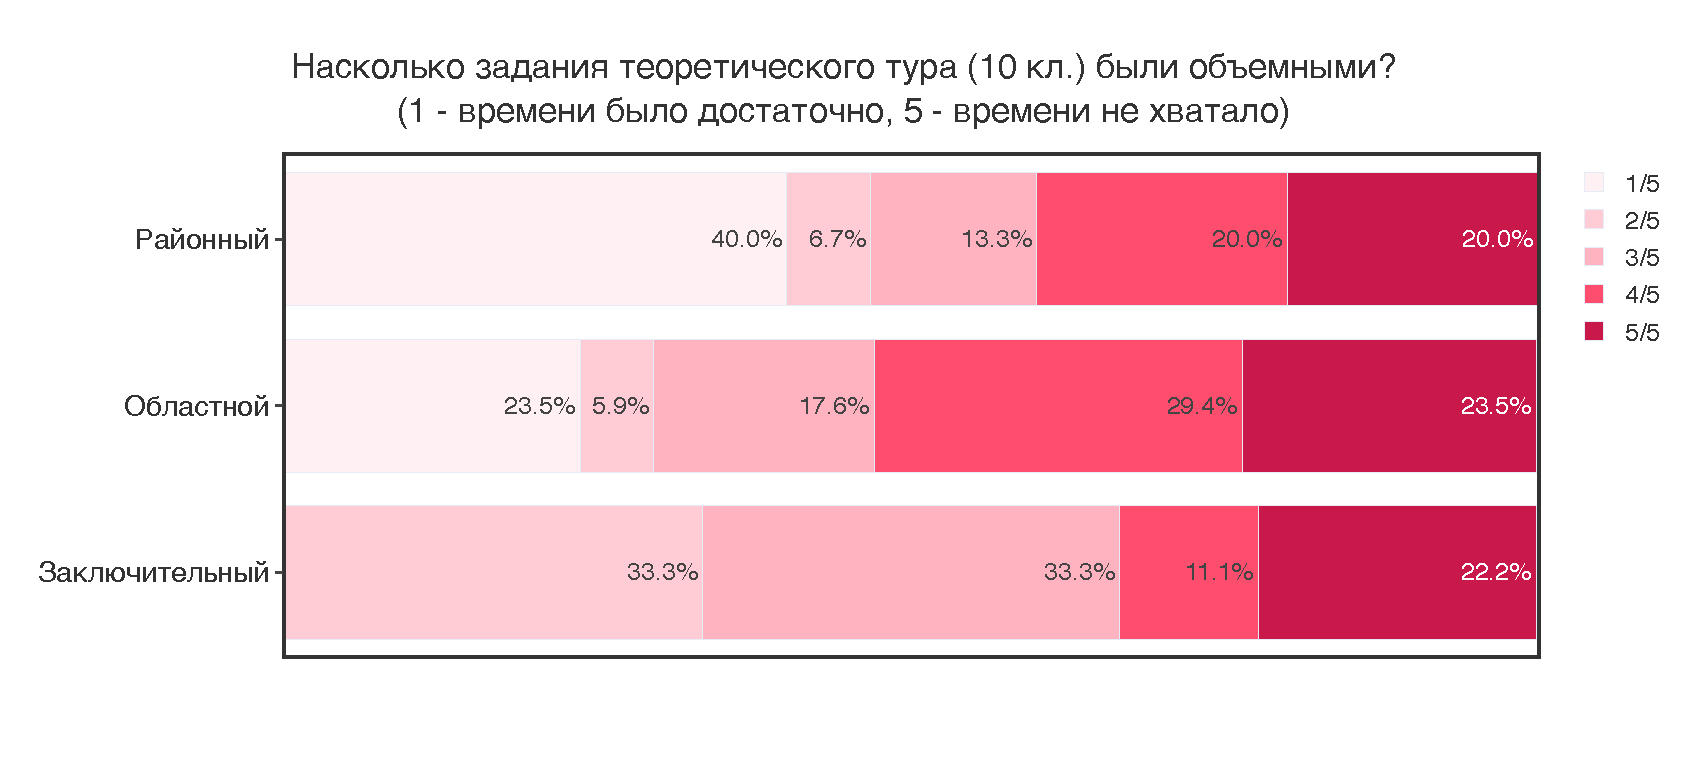
\includegraphics[width=\linewidth]{../export/pdf/demographics/volume-grade10.pdf}

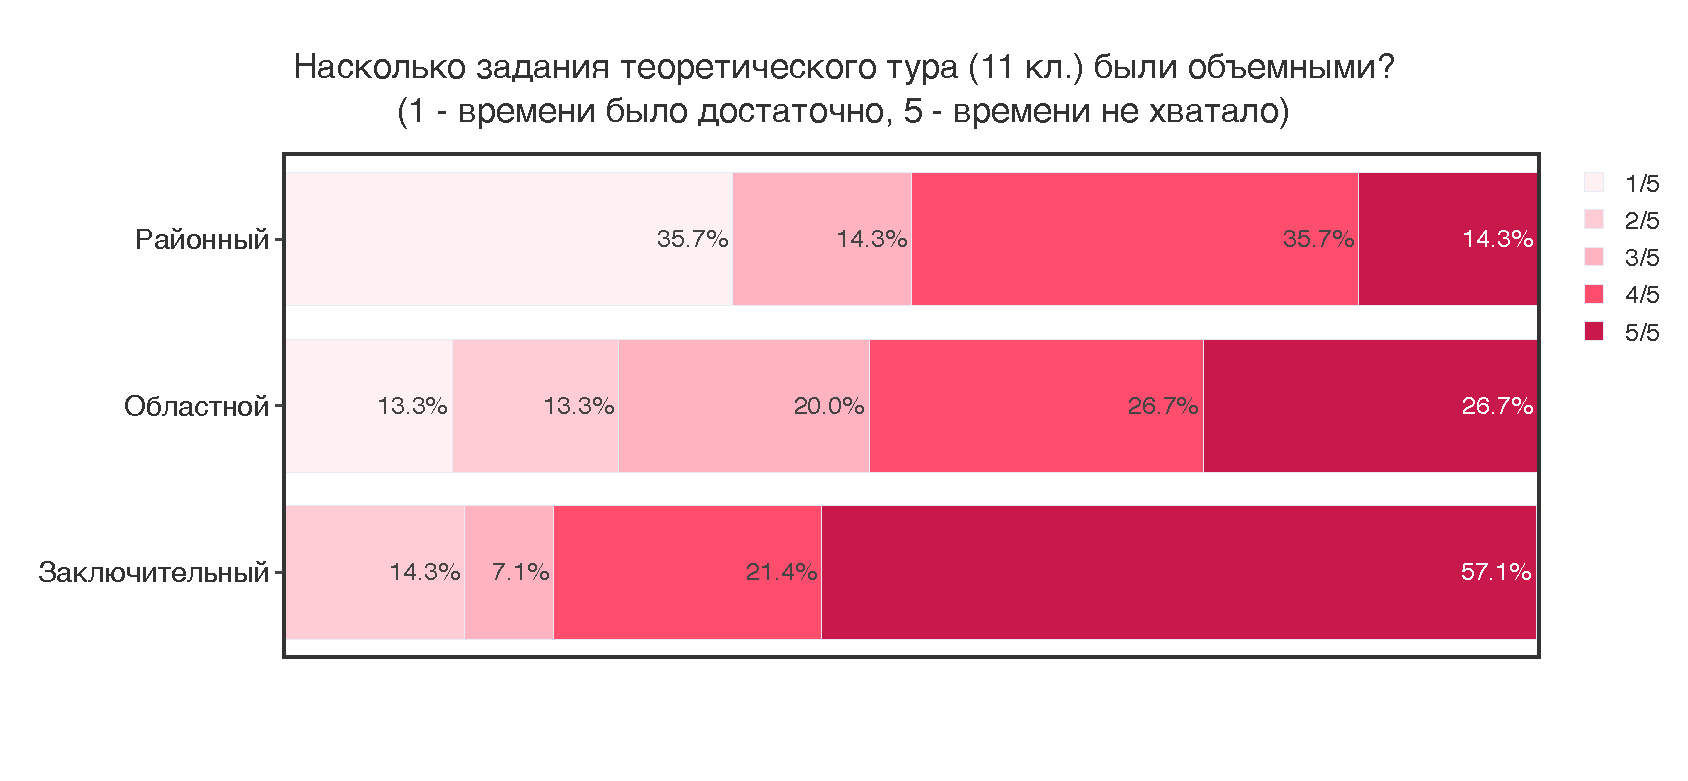
\includegraphics[width=\linewidth]{../export/pdf/demographics/volume-grade11.pdf}

\newpage 

\section{Насколько задания были интересными?}

Участникам олимпиады предлагалось оценить насколько задания были интересными по 5-бальной шкале.

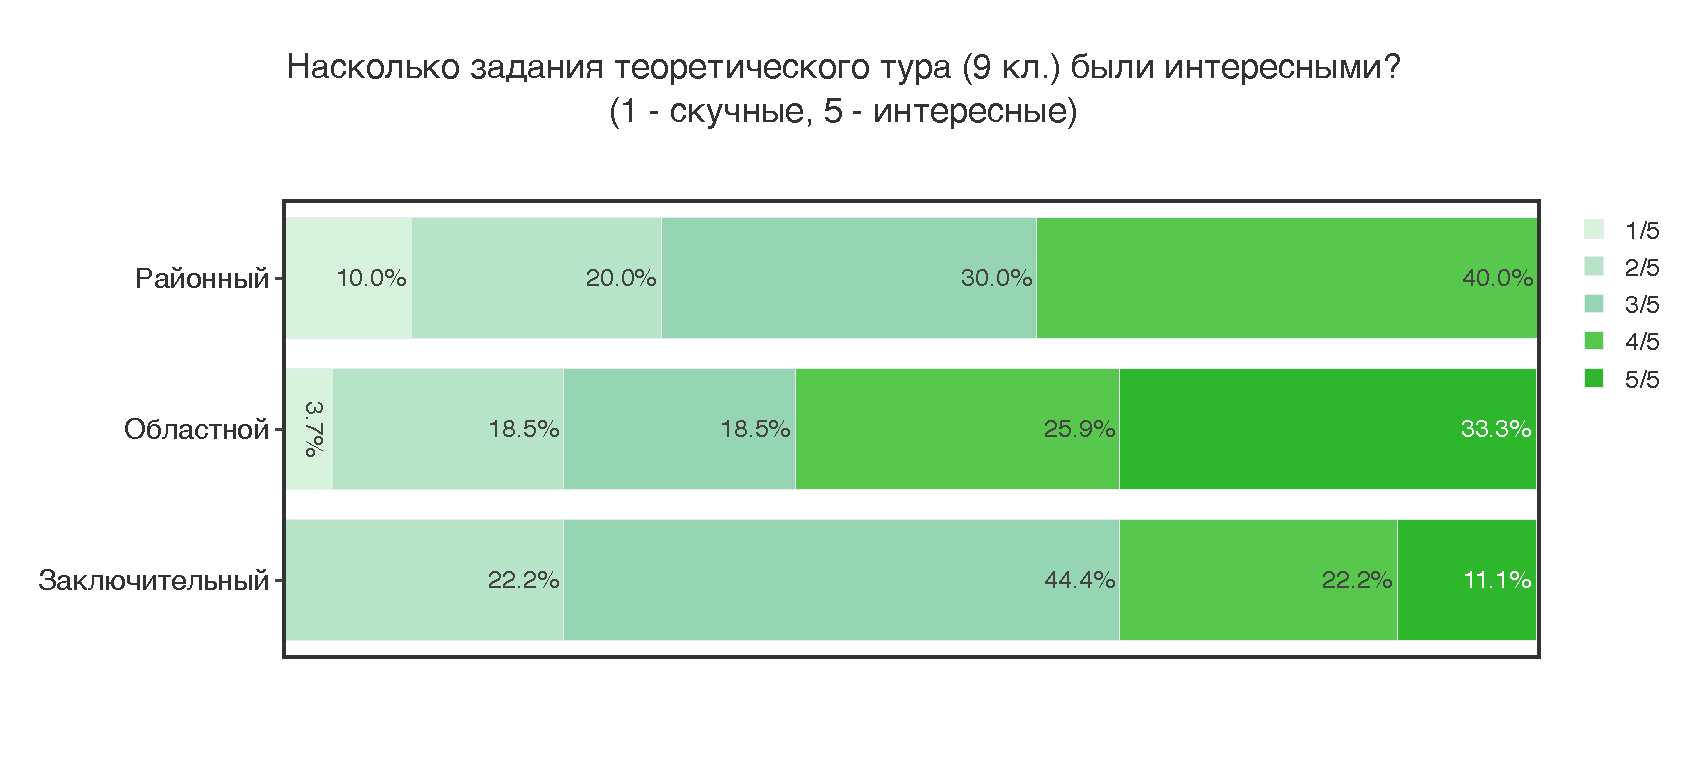
\includegraphics[width=\linewidth]{../export/pdf/demographics/interest-grade9.pdf}

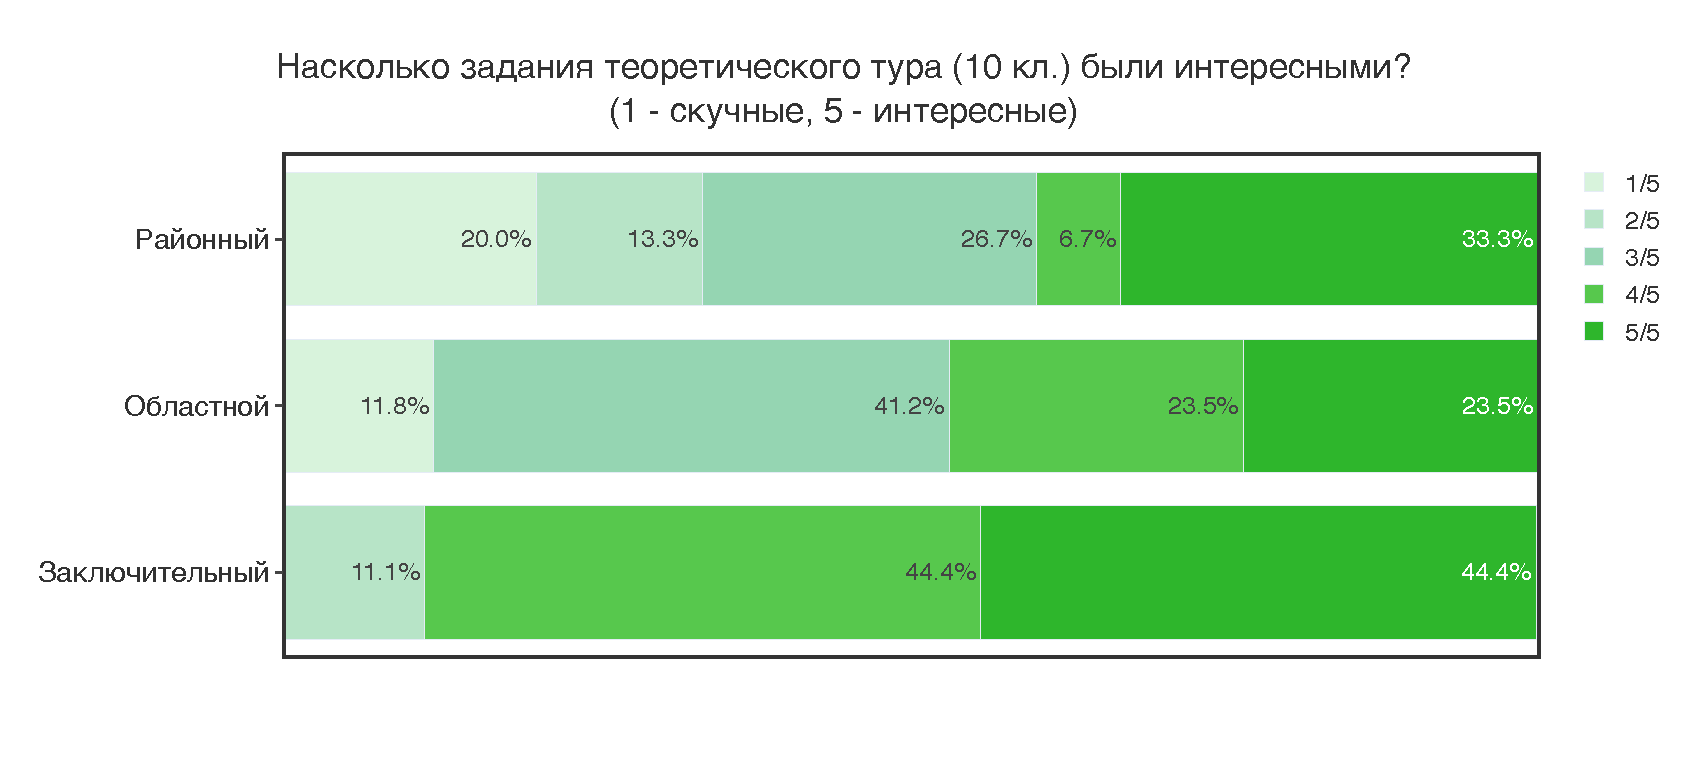
\includegraphics[width=\linewidth]{../export/pdf/demographics/interest-grade10.pdf}

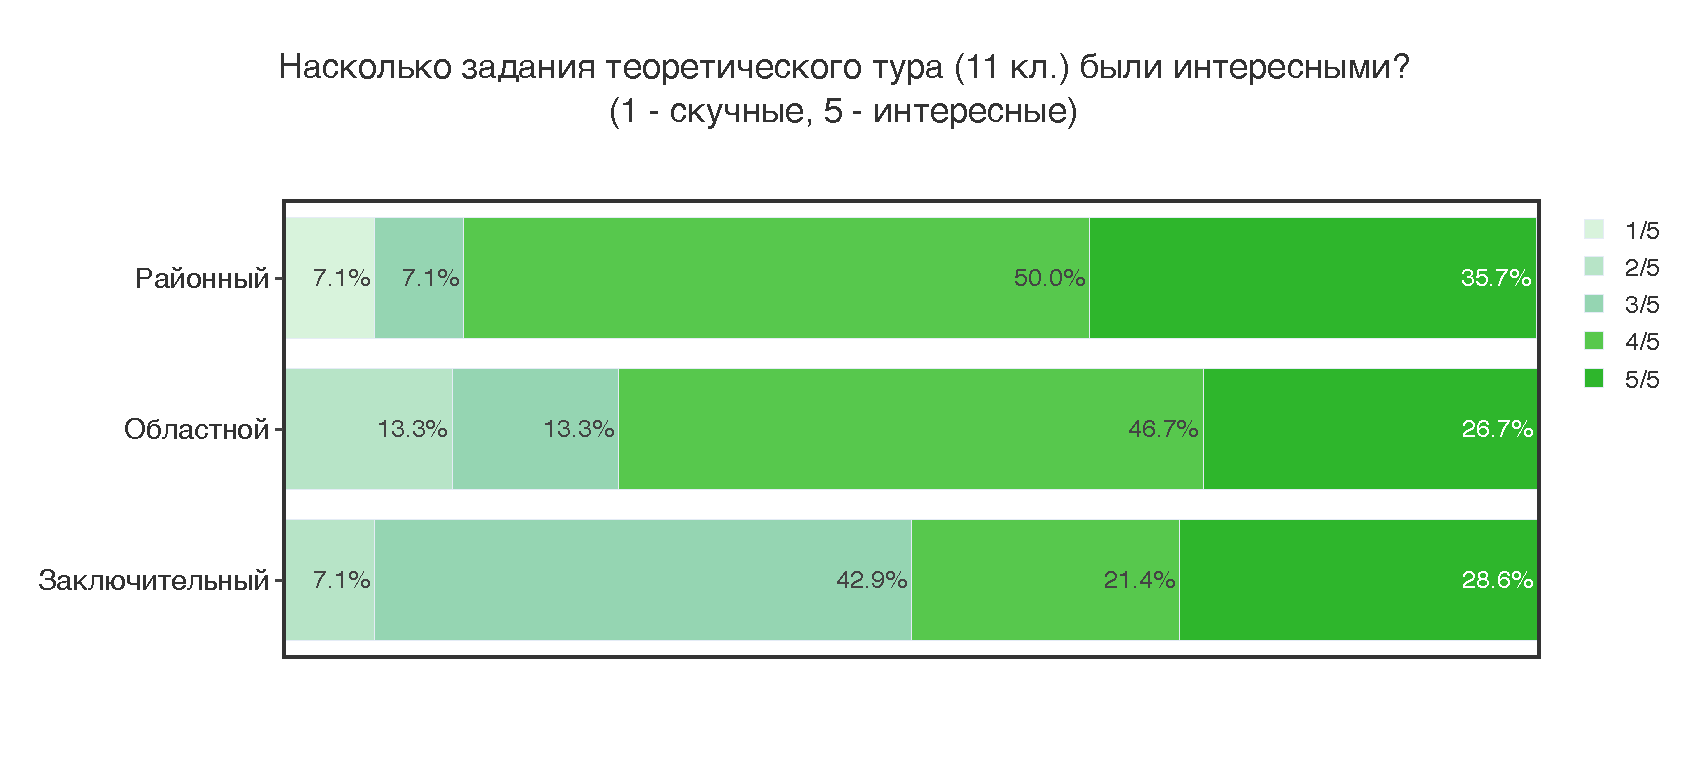
\includegraphics[width=\linewidth]{../export/pdf/demographics/interest-grade11.pdf}


\subsection{Впечатления о районном этапе}
Ученикам предлагалость ответить на следующий вопрос в открытой форме: \textit{Ваши общие впечатления от заданий районной олимпиады? Что понравилось, что не понравилось? Что хотели бы изменить? Скажите все, что считаете нужным сказать.} Орфография и пунктуация респондентов сохранены.

\begin{itemize}
    \itemsep-0.2em
    \item[--] Удивился, так как было легче чем ожидал и чем было на прошлых годах, не понравилось что было задание с титрованием (про кристаллогидрат сульфата никеля)
    \item[--] Жүргіздім. Негізі олимпиада мен мектеп программасыңдағы есептердің деңгейі мүлде сәйкес келмиді. Олимпиада есептері мектеп програмассымен қатар жүргізсе деген өтінішім бар. Себебі олимпиада есептері анағұрлым күрделі.
    \item[--] Думаю все было хорошо продумано. Сложенсть задачек соответствовало уровню районки и по времени все было нормально.
    \item[--] [хотелось бы] усложнить задания, добавить общую химию и глубокие знания неорганической. (\textit{Примечание:} этот отзыв оставлен учеником неспециализированной школы)
    \item[--] Все было отлично
    \item[--] Все хорошо, кроме одного момента, хотелось побольше творчества в заданиях, там например порисовать структуры или применения химии в реальной жизни, с которой мы каждый день сталкиваемся. Ещё не хватило наверное классической для олимпиад органической цепочки или задачи на органику.  
    \item[--] Маған барлығы ұнады, бірақ тапсырмалардың логикасын ұғу қиын болды
    \item[--] Олимпиада была интересной, как и способ подачи материала, в некоторых задачах была излишняя информация, типа задачи \#3, а где-то наоборот, моих знаний не хватило для решения задач. Также не хватило времени, хотя и в аудитории я дописывал один, но думаю другие просто и не пытались. В целом это район мне понравился гораздо больше чем предыдущий, в особенности понравилась последняя задача, думаю задачи на термодинамики с прикладными примерами интересные. \*На задачу \#2 времени просто не хватило , даже не приступил
    \item[--] Мен үшін өте қиын болды
    \item[--] Было немножко трудно, но задание были интересные
    \item[--] Региональные задания были немного проще, чем предыдущие олимпиадные задания, и задания были интересными
    \item[--] Мне было очень интересно
    \item[--] Понравилось : Интересные задачи - Задачи 3, 5 были крайне интересными/интересными соответственно. Полезные задачи - В задаче 4 полезные рассуждения и выводы. То же касается и последнего пункта задачи 5 Не понравилось : Не хватает органики. В прошлом году на районном этапе, была отличная задача на органику (10кл, 5 задача). Чтобы сохранить объем олимпиады, можно было бы заменить органику на задачу 1
    \item[--] Очень интересная олимпиада, только задачи мне кажется легче чем прошлогодние
    \item[--] мне абсолютно все понравилось, все задачи интересные, аж за каждое хваталась. большое спасибо коллегии, за то что они трудятся и за ежегодные авторские задачи.
    \item[--] Задачи были легкими, но думаю так и надо т.к это только районный этап, понравилась 2 задача, сильно напоминает стиль всероссов, хотя щелкается за 5 минут если найдешь азот. В целом задачи довольно легкие решил все примерно за 20-30 минут.
    \item[--] Было достаточно сложно чем я ожидала
\end{itemize}

\subsection{Впечатления об областном этапе}
Ученикам предлагалость ответить на следующий вопрос в открытой форме: \textit{Ваши общие впечатления от заданий областной олимпиады? Что понравилось, что не понравилось? Что хотели бы изменить? Скажите все, что считаете нужным сказать.} Орфография и пунктуация респондентов сохранены.

\begin{itemize}
    \itemsep-0.2em
    \item[--] Задания в довольно часто повторяют идеи районки, но на более высоком уровне, как и идеи на респе в предыдущем году. Последняя задача и задача про серу с галогеном 11 класса показалась гробом в начале решения, но когда находится точка, с который стоит начать, задача упрощается в $10^4$ раз. Понравилось, что давали формулу и константы когда это нужно было, это уравнивает шансы участников и помогает оценить критическое мышление, нежели зубрёшку
    \item[--] Задания видно было классные, но моих знаний на них не хватило 
    \item[--] Задания проще, чем в прошлые годы. Вторая задача интересная
    \item[--] Не понравилось - не было органики
    \item[--] Организация подкачала, а задания интересные,мне понравились
    \item[--] Задачи были довольно скучными и легкими. Надо читать внимательно и все вышло бы(мне кажется)
    \item[--] Думаю в этом году они легче чем в прошлом году. Задачи были интересные
    \item[--] Угадайки были интересными и в меру сложными. Термодинамика(4 задача) была скучная. Электрохимия была интересная и сложнаватая, но объёмная. Органика довольно интересная, но сложная.
    \item[--] Было сложно
    \item[--] Мне очень нравится формат задач. Они были в меру сложными и интересными. Я думаю эти задачи явно повысили мой уровень в их понимании и решении. Формат 3 маленькие и 3 большие задачи очень уместен для организации отведенного времени и увеличения интереса участников олимпиады!
    \item[--] Мне в целом все понравилось, понимаю, куда нужно расти. Задачи интересные, решаемые и заставляющие подумать. Спасибо нашей прекрасной коллегии химиков 
    \item[--] Были нудноваты, прям не было интереса их решать, сухие условия, задача про Мадияра была вначале интерестна, но тоже в какойто момент стала нудной, хоть и довольно много времени уделял решению, вдвое больше чем могло бы понадобиться задаче, всеравно почти уложился в данное время, не было напряжения под конец, а в том что не решил некоторые задачи, виной моя халатность при подготовке.
    \item[--] общие впечатления - надо было больше готовиться. а если серьезно, то в какой-то степени даже обрадовалась, что пришли решабельные задачи. единственное, что не изменилось с прошлой области, так это органика. вечно оставляю ее на потом из за сложности и нехватки времени.
    \item[--] Мне понравились все задачи, хотел поблагодарить коллегию за эту олимпиаду
    \item[--] Задания были довольно интересными по содержанию, но задания 5,6 сложноваты. Можно было бы сделать чуть легче
    \item[--] Именно к составлению задач не имею претензий. А на место проведения есть много вопросов.
    \item[--] Задачи было сложными и интересными
    \item[--] Задания были значительно легкими по сравнению с прошлыми годами. Решабельные задачи. Не понравилось, что потеряла 30 минут из-за низкого подключения сети к вайфай на олимпиаде. А это время мне никто не вернул.
    \item[--] Интересные задания, было легче решать чем в прошлом году. А органика была посложнее
    \item[--] Есть и легкие и трудные задачи, но как по мне для хорошего олимпиадщика не составило бы проблем набрать как минимум 40 из 70.
    \item[--] Задания довольно таки интересные, однако в виду незнания по каким разделам необходимо готовиться , было сложно. Было бы не плохо если бы задания были более менее для уровня средних школ и гимназий, хоть я и являюсь учеником гимназии , однако у нас нет такого времени и возможности, чтобы посвящать себя полностью олимпиаде, так как по всем остальным предметам пишем Сор и Соч, а после обеда есть дополнительные занятия кружкового характера, и наши учителя также не всегда свободны, чтобы дополнительно на нас переключать свое внимание, как достаточно взрослый понимаю их высокую нагрузку. Учителя максимально стараются дать все необходимые знания , однако по вышесказанным причинам , полагаю у них нет возможности всецело посвятить себя подготовке к олимпиаде. (надеюсь, что все учителя такие как в нашей 40 гимназии, стараются максимально нас направить и подготовить к олимпиадам, а также качественно проводить уроки)
    \item[--] самая худшая областная честно
    \item[--] Весьма скучная, но и долгая, прикольных задач не видел
    \item[--] БОЛЬШОЙ РАХМЕТ ЗА ЗАДАЧИ
    \item[--] В целом впечатление от олимпиады хорошее. Не считая однообразных вычислений в 4 задаче, все задачи были интересными. Понравилось более нестандартная (как мне показалось) формулировка пунктов по аналитике во второй задаче
    \item[--] Честно говоря в этом году задания для меня показались легче. Потому что до этого я сидела и минутами не могла понять что просит от меня задача. А в этом году начиная с первого по пятые задачи (кроме органики и второй задачи про неизвестные вещества) были очень даже доступными. чтобы получить максимальные баллы. Лично у меня траблы были с частью где нужно выводить реакции и тд. Потому что по этой части у меня совсем мало опыта, и за это у меня отнимали баллы. А по математической части мне все понравилось.
    \item[--] На мой взгляд, задания 1 тура надо разделить и часть оставить на 2 тур , так как время , данное на 1 тур, слишком маленькое ( 4 часа ,хотя должно минимум 6 часов) , в то время как 2 тур выполняется за 30-40 минут. ( макс. 1 час) Насчет заданий, мне хотелось бы узнать, из каких источников вы берете материал для составления задач, так как я считаю что задания были слишком сложными ( соответствуют 2-3 курсу университета, и нужно максимально сконцентрироваться на изучение химии, чтобы получить хорошие баллы, что это довольно трудно для меня как современного подростка) Спасибо за понимание!
    \item[--] Мне понравились все задачи, они более логичные чем теоретические
\end{itemize}

\subsection{Впечатления о заключительном этапе}
Ученикам предлагалость ответить на следующий вопрос в открытой форме: \textit{Ваши общие впечатления от заданий республиканской олимпиады? Что понравилось, что не понравилось? Что хотели бы изменить? Скажите все, что считаете нужным сказать.}. Орфография и пунктуация респондентов сохранены.

\begin{itemize}
    \itemsep-0.2em
    \item[--] В целом впечатления о комплекте заданий очень положительные, видно что жюри постарались сделать задания как можно более интересными. Темы заданий были достаточно разнообразными. Единственное, что мне не понравилось, это неявность пунктов в задачах Блиц Физхимика и Намешали. Не увидев в пунктах задачи требования обосновать свой ответ, я посчитал ненужным предоставлять обоснования к своим ответам, особенно учитывая, что пункты задач были сформулированы как закрытые вопросы. Думаю, многие учащиеся, включая меня, предоставили более развернутые ответы на вопросы, если бы это требование было прописано более очевидно в условии задач. Помимо этого, мне показалось, что возможно марк схема по данным задачам была черезчур придирчивой, но с другой стоионы, я понимаю, что ученик предоставивший более полное и правильное обоснование в своем ответе звслуживает больше баллов. Тем не менее, я остаюсь при своем мнении о неочевидности требования предоставить обоснования к своим ответам в этих задачах.
    \item[--] Мне очень сильно понравились задачи на физхимию (4 и 5), в которых надо было использовать логику и мат. аппарат. Эти задания, особенно пятая, довольно близки к самой науке, что сподвигло меня кликнуть и прочитать прикрепленные научные статьи. Именно такие задачи, на мой взгляд, пробуждают интерес у учеников не только к химии, но к науке в целом. Скорее всего единственный минус таких задач в том, что на апелляции выстраивается очередь до 50 человек даже после 4 часов. Это скорее к организации, но думаю есть способ сделать ответы неоспоримыми и однозначными. Смотря на задачи, я понимаю какой это большой труд делать такую работу, но меня все еще не покидает мысль, что их можно как-то улучшить, добавить какие то детали, сделать более интересными и запоминающимися. Буду продолжать думать насчет этого...
    \item[--] Задания хорошие, но чувствуется колоссальное различие в сложностью с задачами прошлых лет на респе. Задачи заставляли задуматься в ином ракурсе нежели другие химические задачи, что кому-то понравилось, а кому-то нет, лично мне понравилось, ведь оценивает как кругозор, так и умение мыслить.
    \item[--] Задания составлялись больше на знание хорошей математичкского аппарата нежели что то химияеское или логичное. Последнее задание казалось особо нелогичным, а 7ое буквально не давало шанса на хороший балл без зубрежки (допустим) Алексеева. Лично мне больше всех понравилась 2ая задача (про кобальт) и 4ая более менее на логику.
    \item[--] Задачи не сбалансированы, 6 неорганик и 1 физхимия. Не лучше ли было сделать 4 неорганики, 1 органику, 1 физхимию и 1 аналитику. Баллы не сбалансированы, за расчеты которые занимали пол страницы могли дать столько же, а иногда и меньше баллов чем за какую-то одну реакцию. Были задачи в которых стоит тебе ошибиться лишь в 1 реакций, то за задачу сразу 0, несмотря на то, что идей и многое другое почти идентично с правильным решением. 
    \item[--] Имхо, в этом году ты должен был, именно знать некоторые вещи. Реакций с кровяной солью, электролиз оксалата, и тп. Если честно прошлые года (2019-2022) были намного легче для меня (набирал 80\%). Я жутко занервничал и написал плохо. Хотелось бы, чтобы в задачах нужно было меньше знать и можно было вывести все самому.
    \item[--] Думаю надо включать задачи с разных тем химии. Аналитика, физхимия, общая химияи тд. Прикольно было то что участников проверяли с разных областей. По типу математики, анализирующей точки, на мировоззрение.
    \item[--] Очень понравились переплетение математики и физики на олимпиаде то есть не только знание химии нужны чтобы решить нужно иметь хоть какие то знание по математике. Не понравилось то что задачи были очень громозкими для всех. Все получили маленькие по отношению общему числу баллов
    \item[--] Задания были интересными, но вторая задача у 11 класса с комплексами (хорошо, что не моими) была тяжёлой, кто ее решал тот не успел решить остальное
    \item[--] Вроде все нормально, т.к это была моя первая офф олимпиада было огромное давление, и не смог написать на свой максимум(как и все).
    \item[--] Если учитывать, что это респа, то справедливо. Я готовился к респе по прошлым годам, и этот год был крайне другой. И стиль задач будто изменился колоссально(если просто посчитать средний балл прошлого и этого года на 1 туре). 
    \item[--] Задания были в некоторых моментах не продуманы до конца в плане деталей, ведь диапазон ответов был широким и несколько вариантов ответа были возможны. Более того, задания были существенно труднее среднестатистического уровня сложности республиканских олимпиад.
    \item[--] Мне кажется, задачи были слишком объемными; 5 часов с учетом стресса не хватало никак. Одна задача занимала 3 страницы, на чтение условии ушло полчаса. В целом, формат с прошлой респы слишком сильно изменился (не говорю, что это плохо, но желательно видеть плавный переход). Две из 8 задач были сделаны в стиле Всероссийской, к чему никто не был готов. В этом году, честно, разочаровалась в задачах, тк многие описания были на знания, нежели на понимание концепта. В прошлых годах можно было решить парочку задач с помощью логики, вчитываясь в условия задач, однако в этому году логика видимо не проверялась.
    \item[--] Очень тяжелые и непонятные,или я просто плохо знаю химию
    \item[--] думаю каждый писал об этом - задачи гроб, но, наверное, это из-за упавшего уровня знаний учеников. Задачи по сравнению с прошлым годом вводят в дизмораль с первых минут, но они необычные и очень интересные. Так как я не готовился к Олимпиаде, не могу сполна оценить их, но сделав вывод со слов других учащихся - думаю стоило бы добавить подсказок. Понравились задачи, но не понравилась их сложность. После олимпиады меня переполняли чувства заинтересованности (в науке), усталости и сильнейшего разочорования в себе) Составителям печенек
    \item[--] Слишком много неорганики, мало физ хим. и не было аналитики. Не было много тем с силлабуса.
    \item[--] Задачи конечно не легкие,но скучные. Понравилась последняя задача только и 6 была интересная, но за нее по нулям скорее всего. Надеялась еа аналитику и органику, не было в итоге ничего
    \item[--] слишком много баллов за легкие задачи, зачем они вообще на респе, 4-7 классные
    \item[--] Республиканская олимпиада была сложнее предыдущих по моим ощущениям. Возможно, из-за подготовки я часто смотрел решения и считал ее легкой, однако эти задания что-то с чем-то. Особенно 6 задача (9кл) на монетку. Слишком мало информации, как по мне. 7 задачу не стоит винить в сложности. Пункт с BF3 и сродством к электрону для меня совсем новая, было бы интересно решить, если бы не усталость и нехватка времени. Впринципе, олимпа норм как для уровня респы. Но организация хромает.
\end{itemize}

\chapter{Результаты РО}
\section{Распределение баллов}

\subsection{Областной этап}
Задания областного этапа можно скачать с \href{https://olympiads.bc-pf.org/chemistry/oblast/2023}{Базы Olympiads}. Во всех графиках баллы представлены в виде \% от максимального. Довольно удивительно, что несмотря на то, что подавляющее большинство участников посчитали задания областного этапа довольно легкими, баллы сконцентрированы в районе нуля и нормальное распределение на наблюдается (несмотря на довольно большую выборку: 432 результата в 9 кл., 347 в 10 кл. и 312 в 11 кл.).

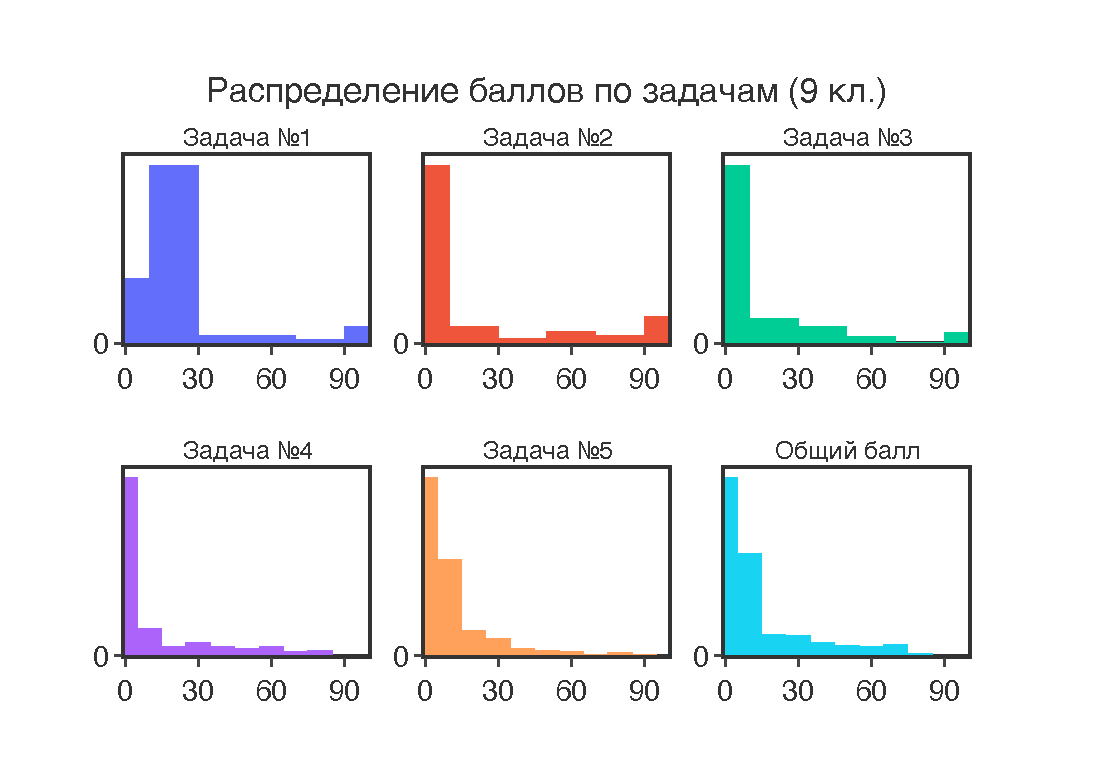
\includegraphics[width=\linewidth]{../export/pdf/results/2023/oblast/grade9-dist-problemwise.pdf}
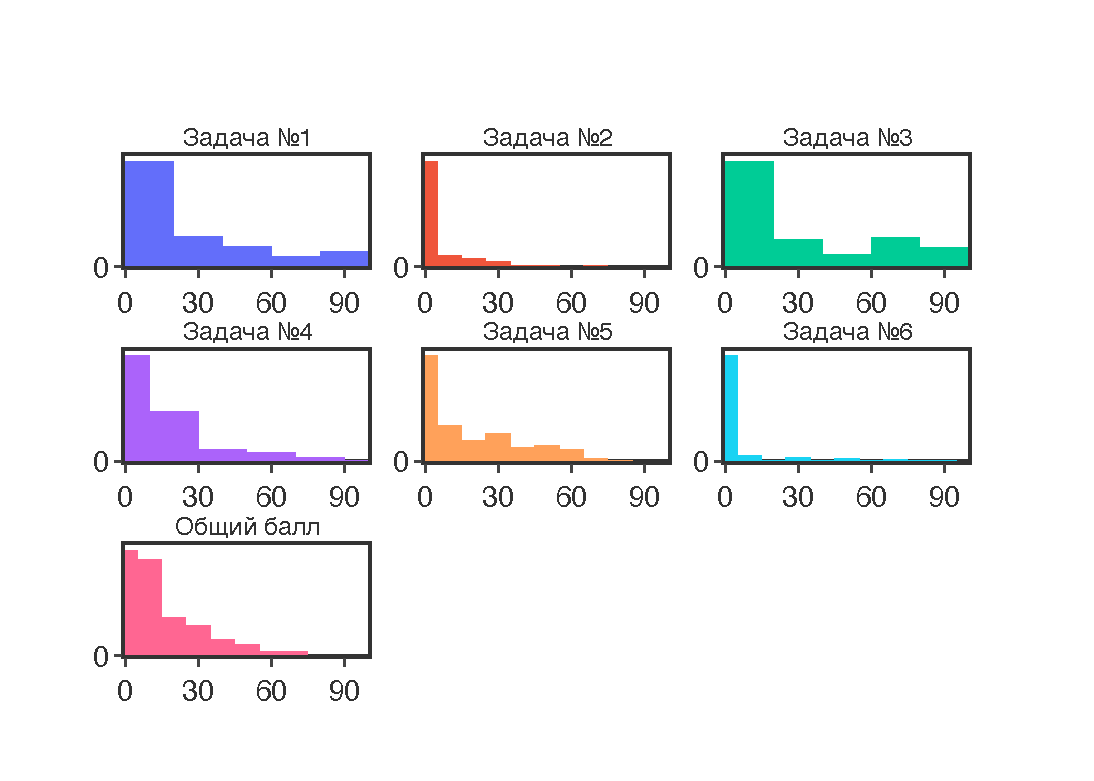
\includegraphics[width=\linewidth]{../export/pdf/results/2023/oblast/grade10-dist-problemwise.pdf}
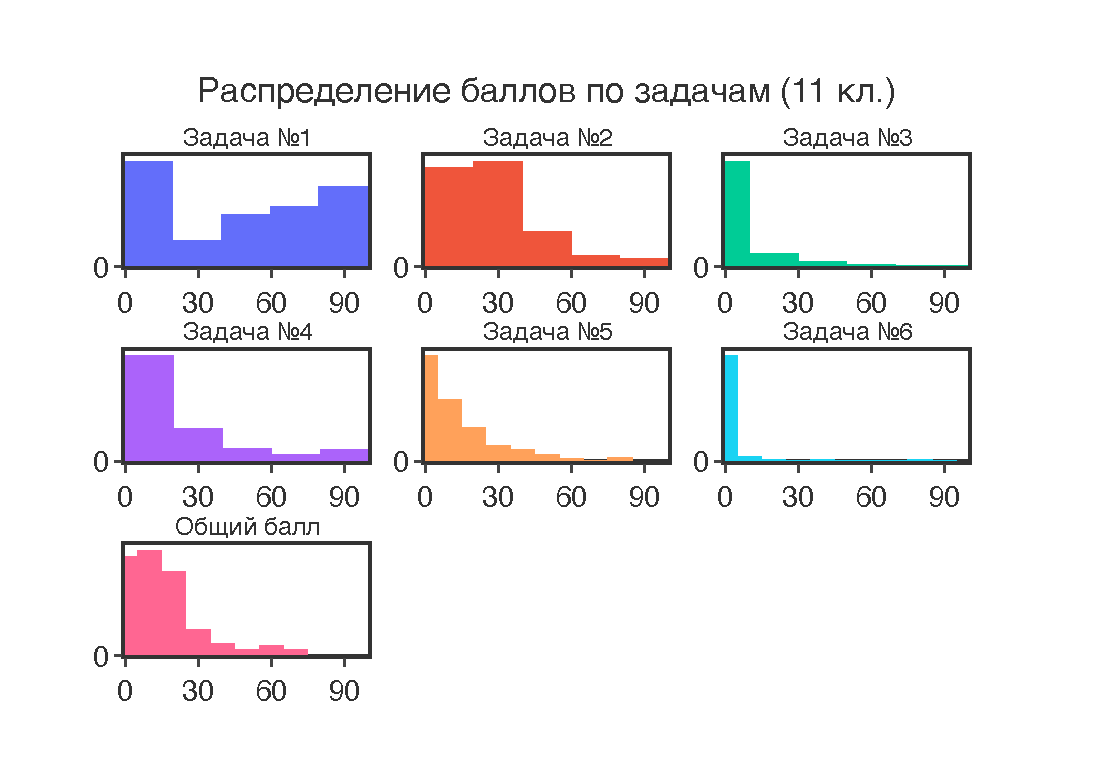
\includegraphics[width=\linewidth]{../export/pdf/results/2023/oblast/grade11-dist-problemwise.pdf}

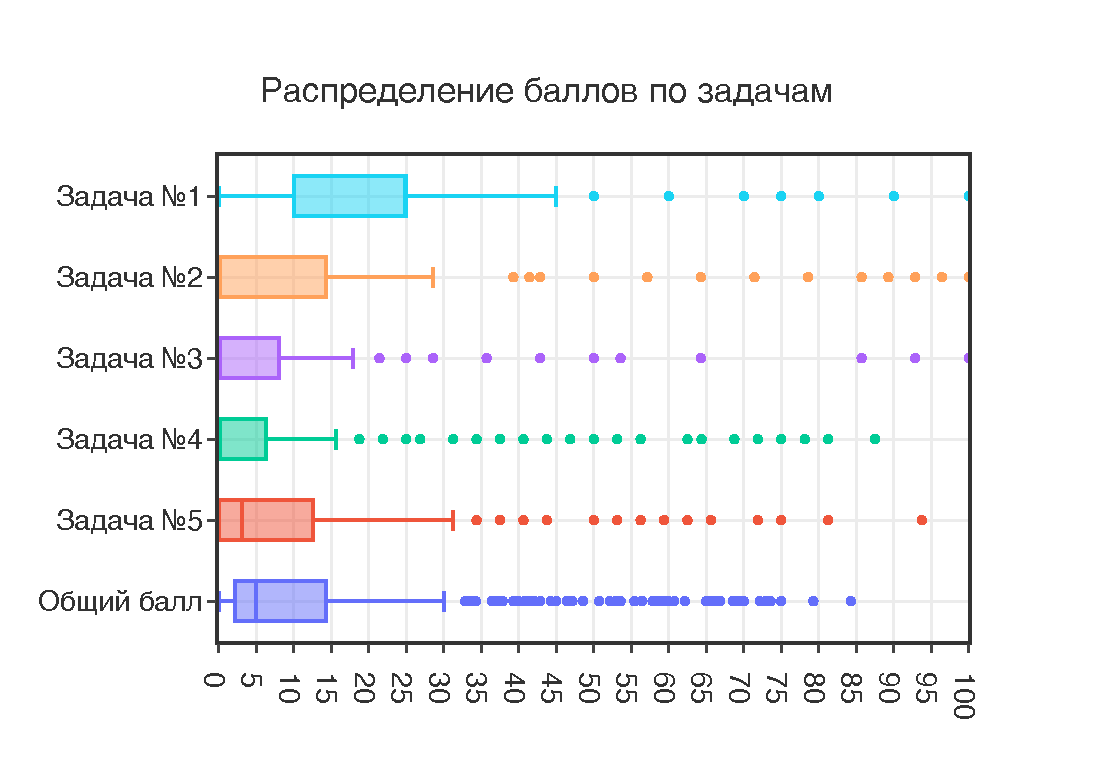
\includegraphics[width=\linewidth]{../export/pdf/results/2023/oblast/grade9-dist-box.pdf}
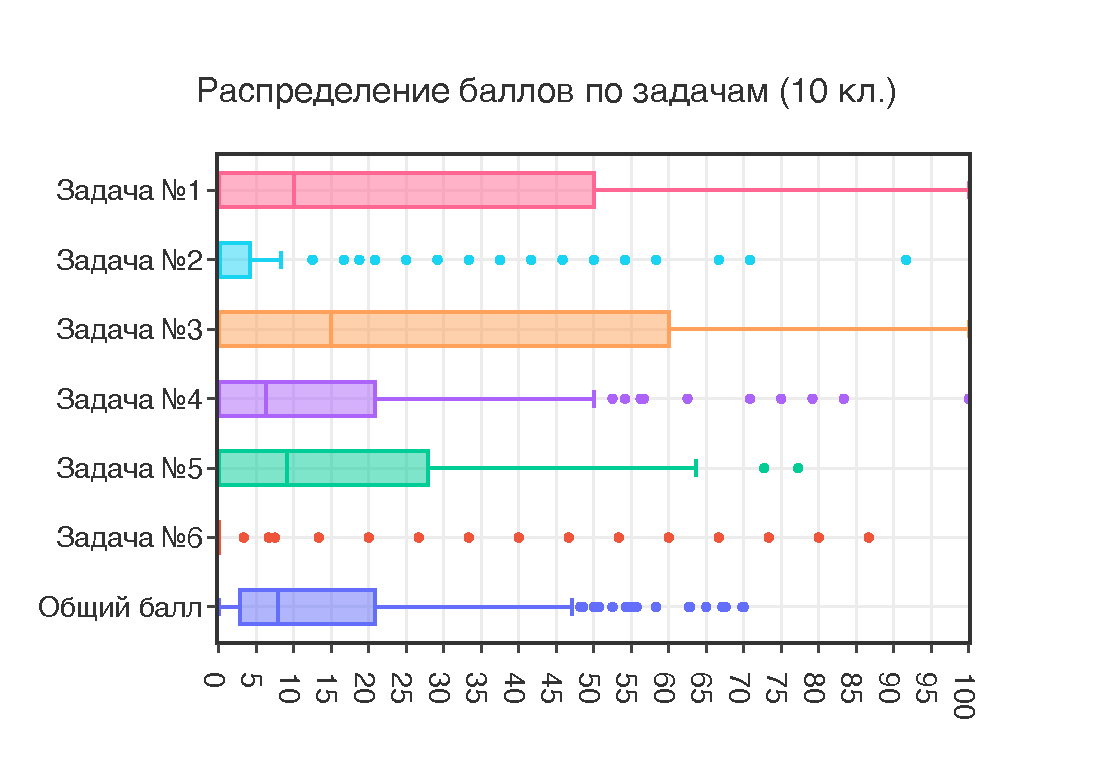
\includegraphics[width=\linewidth]{../export/pdf/results/2023/oblast/grade10-dist-box.pdf}
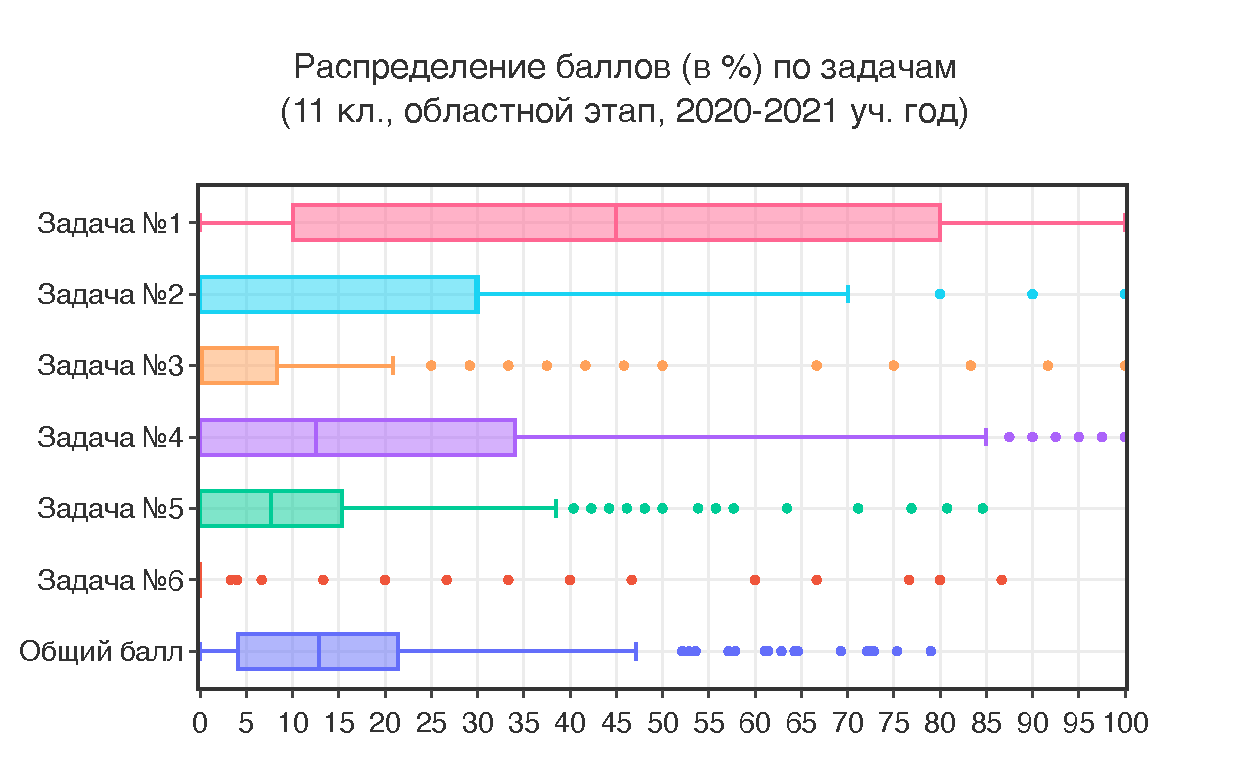
\includegraphics[width=\linewidth]{../export/pdf/results/2023/oblast/grade11-dist-box.pdf}

Создание этих графиков стало возможным благодаря тому, что РНПЦ Дарын, впервые в истории, начал публиковать протокола областного этапа в общем доступе. К сожалению, у протоколов нет единого формата, некоторые области публиковали только итоговые баллы, половина протоколов была опубликована в PDF формате (из-за чего пришлось потратить десяток часов на перенос результатов в формат таблицы) - но все же это положительный шаг в сторону большей прозрачности олимпиад, и Коллегия выражает благодарность за это. 

\subsection{Заключительный этап}

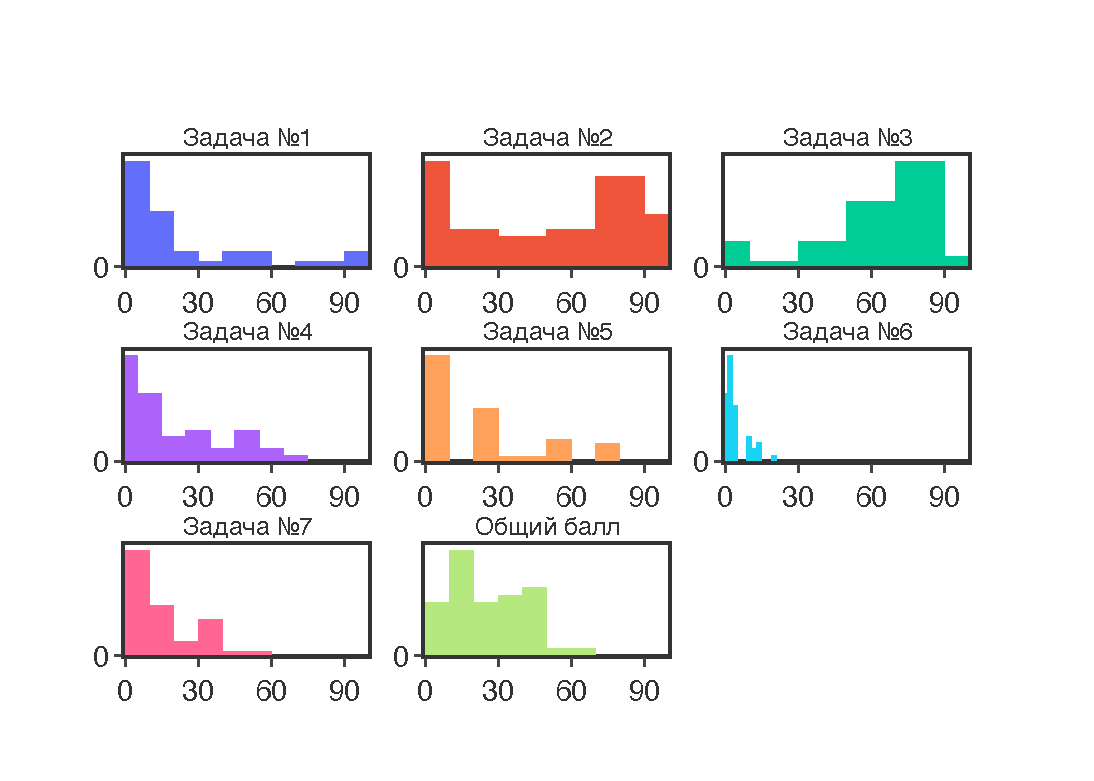
\includegraphics[width=\linewidth]{../export/pdf/results/2023/respa/grade9-dist-problemwise.pdf}
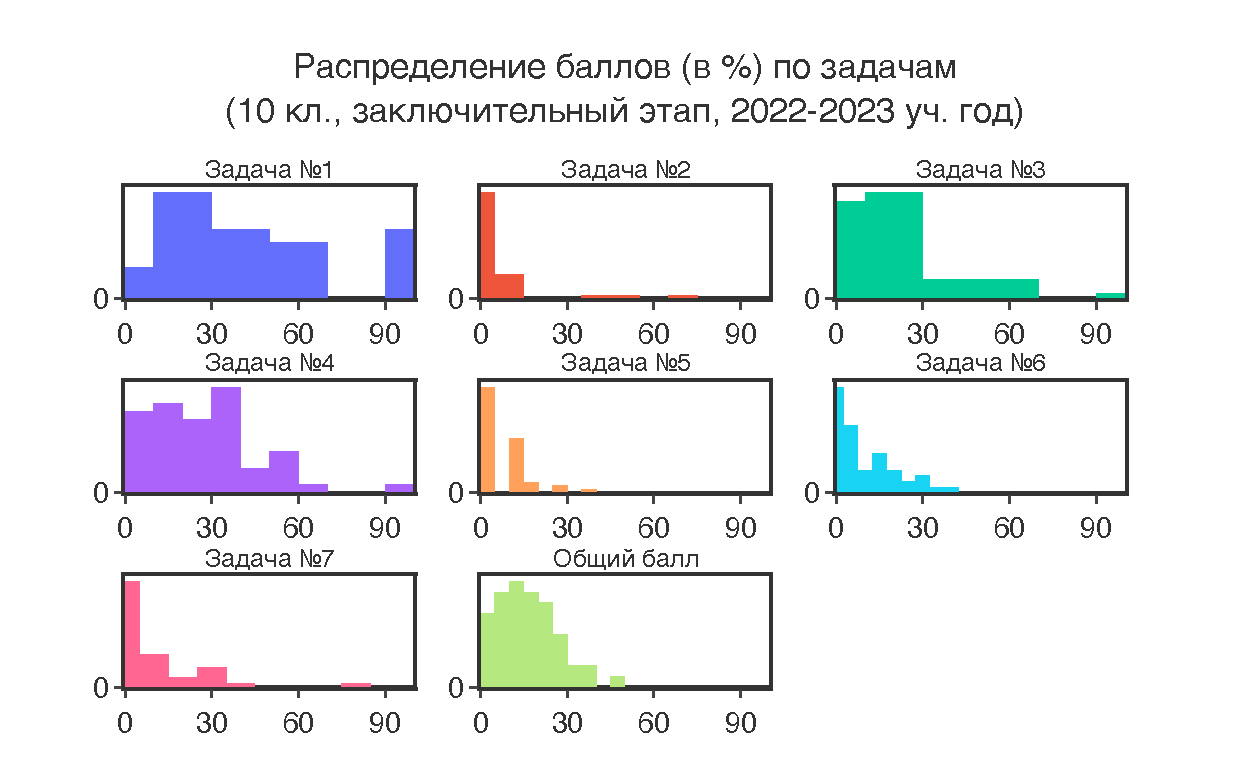
\includegraphics[width=\linewidth]{../export/pdf/results/2023/respa/grade10-dist-problemwise.pdf}
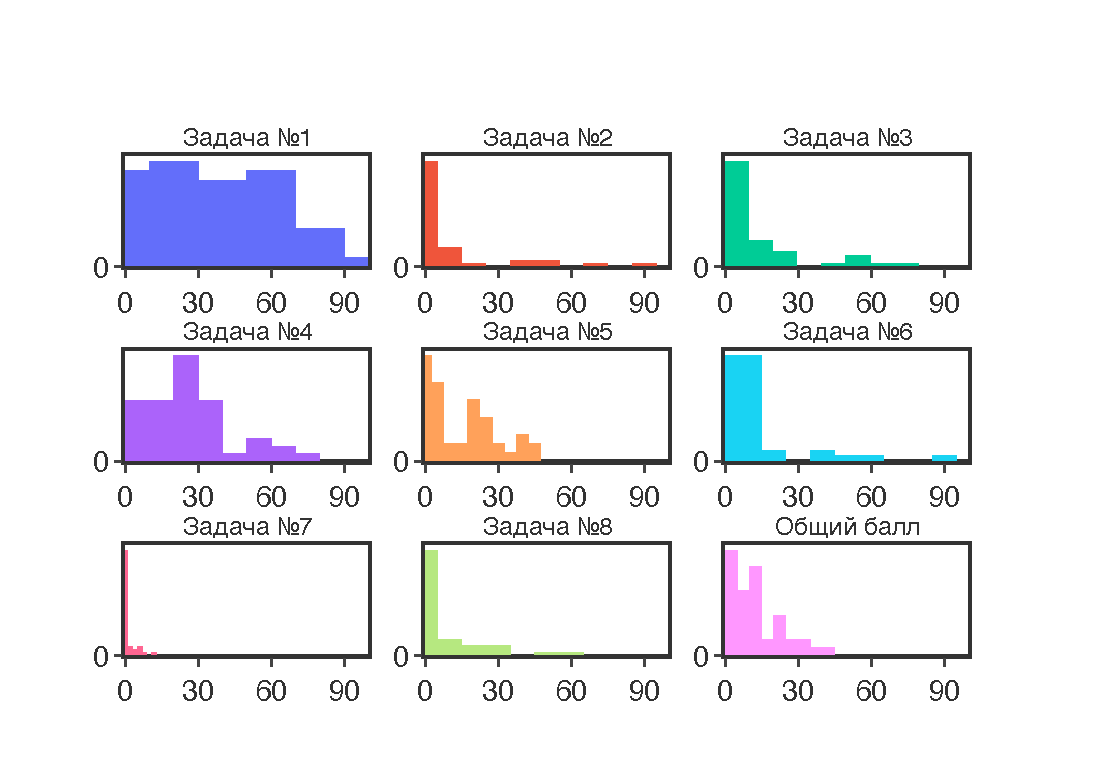
\includegraphics[width=\linewidth]{../export/pdf/results/2023/respa/grade11-dist-problemwise.pdf}


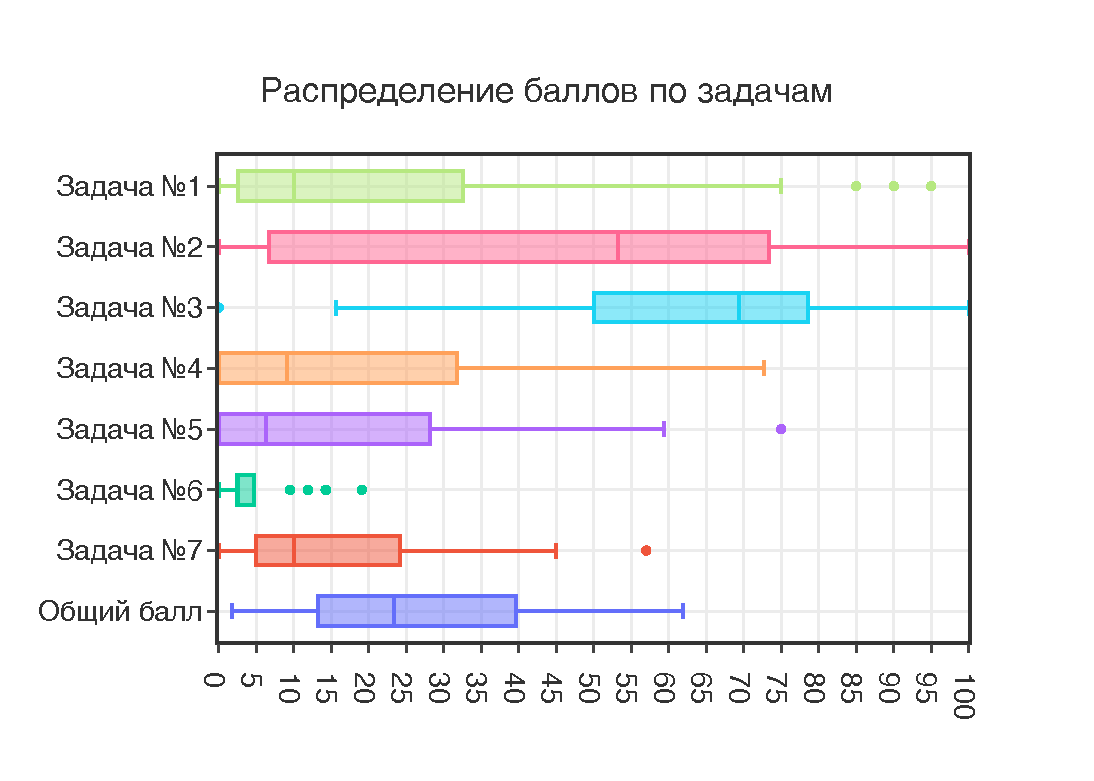
\includegraphics[width=\linewidth]{../export/pdf/results/2023/respa/grade9-dist-box.pdf}
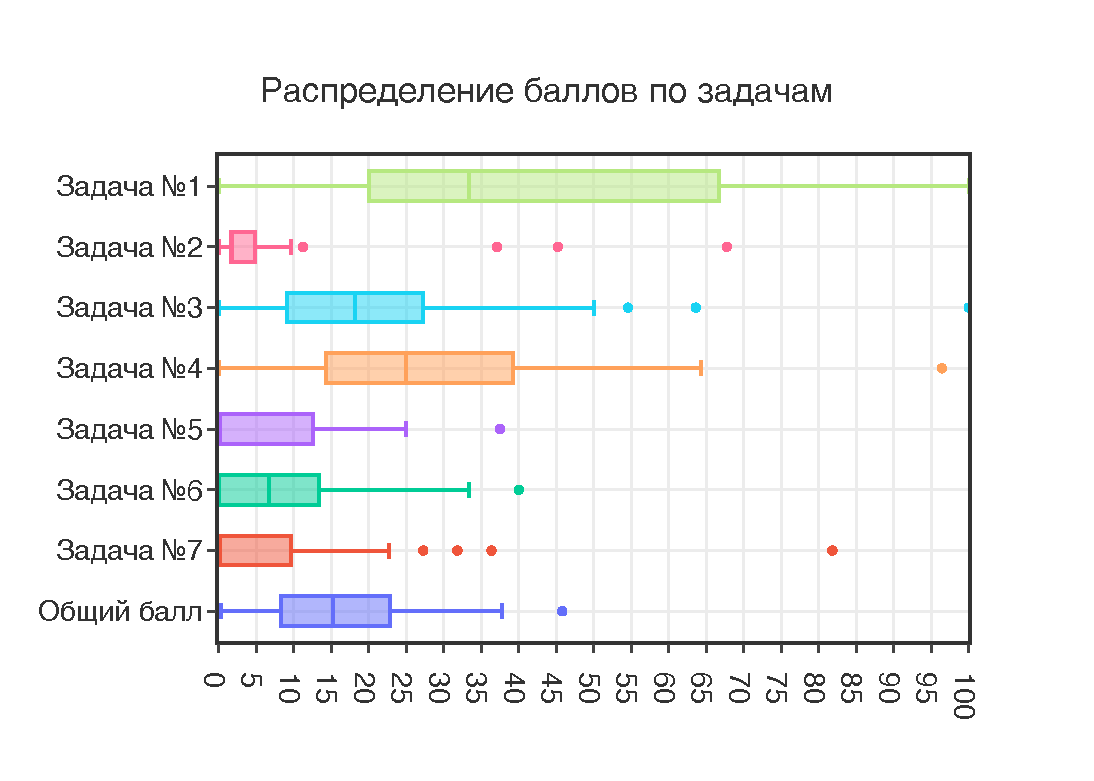
\includegraphics[width=\linewidth]{../export/pdf/results/2023/respa/grade10-dist-box.pdf}
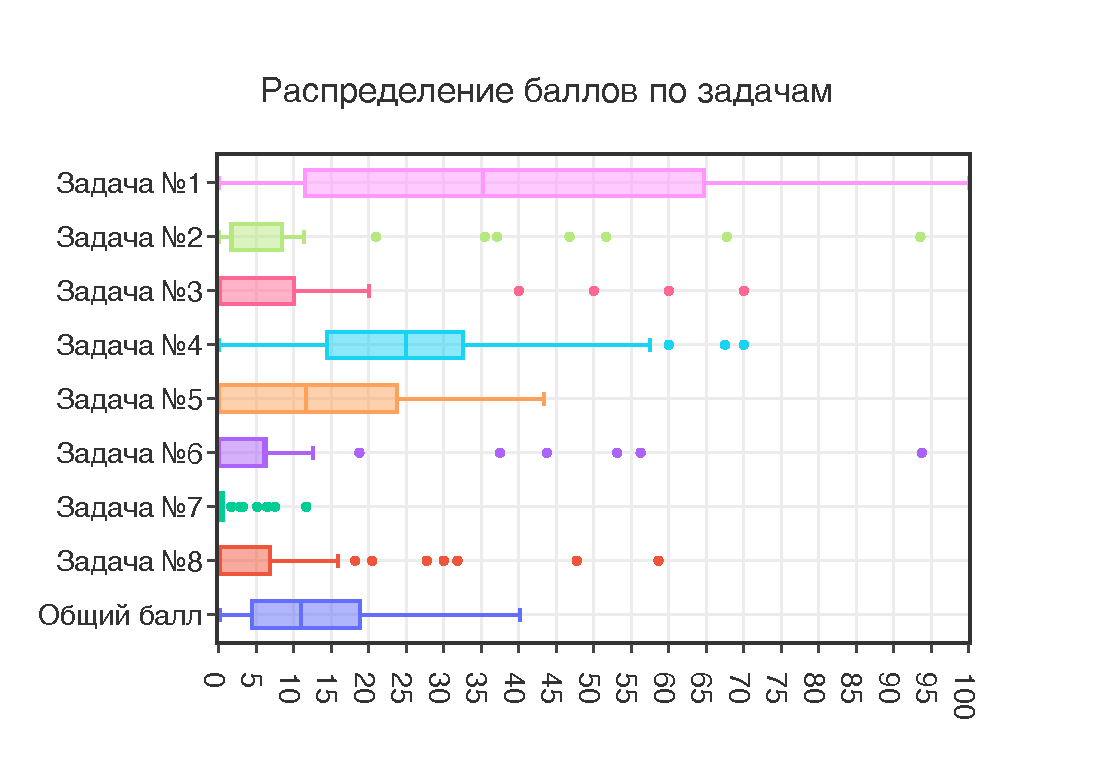
\includegraphics[width=\linewidth]{../export/pdf/results/2023/respa/grade11-dist-box.pdf}

\subsubsection{Результаты 2021-2022 уч. года}

Поскольку не мало участников заключительного этапа считает, что заключительный этап в 2022-2023 уч. году был значительно сложнее заключительных этапов в предыдущие годы, мы решили построить аналогичные графики для результатов 2021-2022 и 2020-2021 уч. годов.

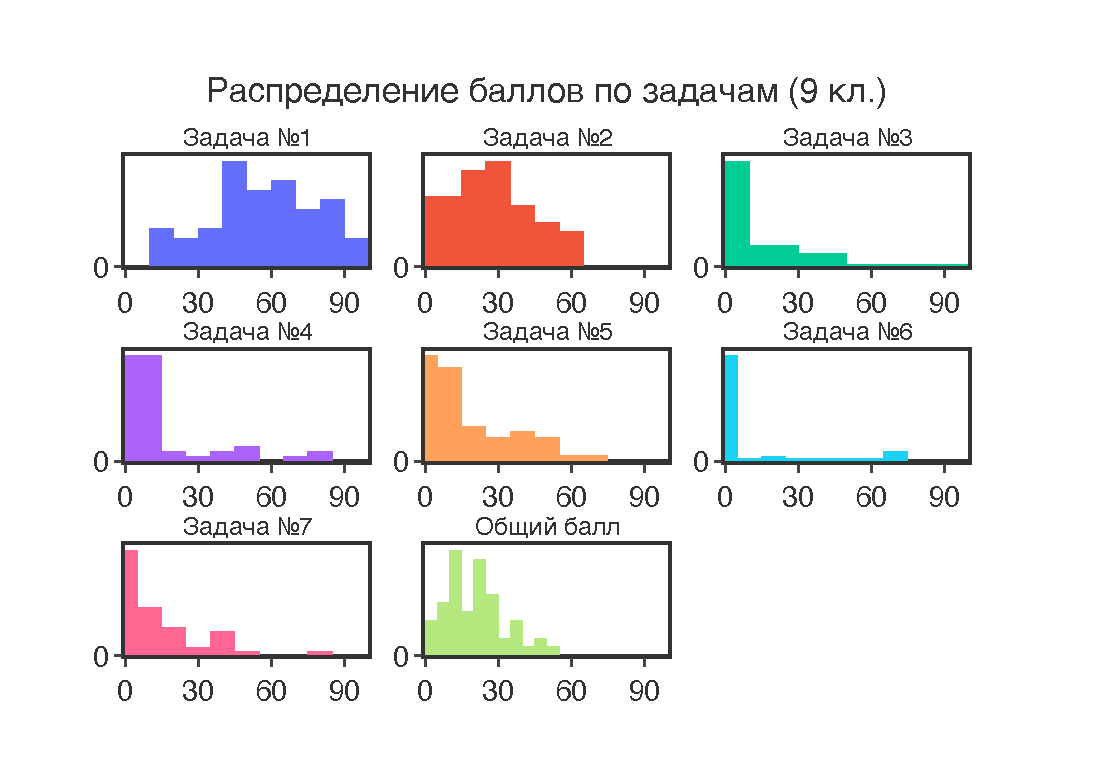
\includegraphics[width=\linewidth]{../export/pdf/results/2022/respa/grade9-dist-problemwise.pdf}
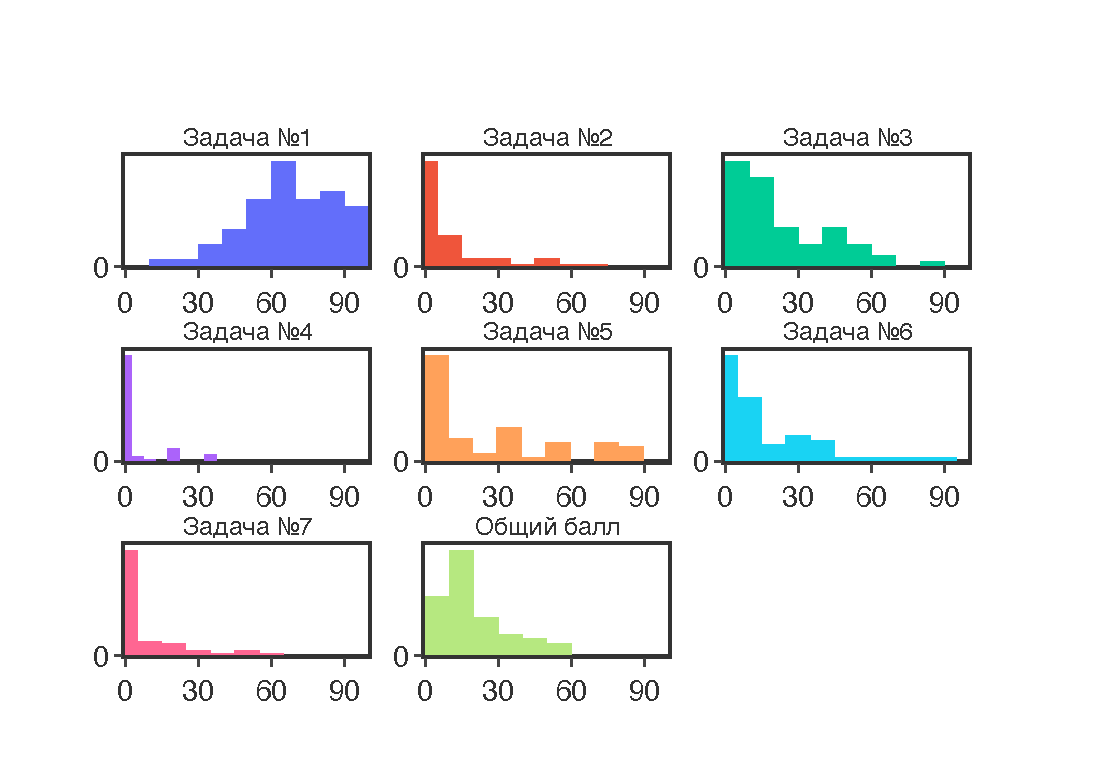
\includegraphics[width=\linewidth]{../export/pdf/results/2022/respa/grade10-dist-problemwise.pdf}
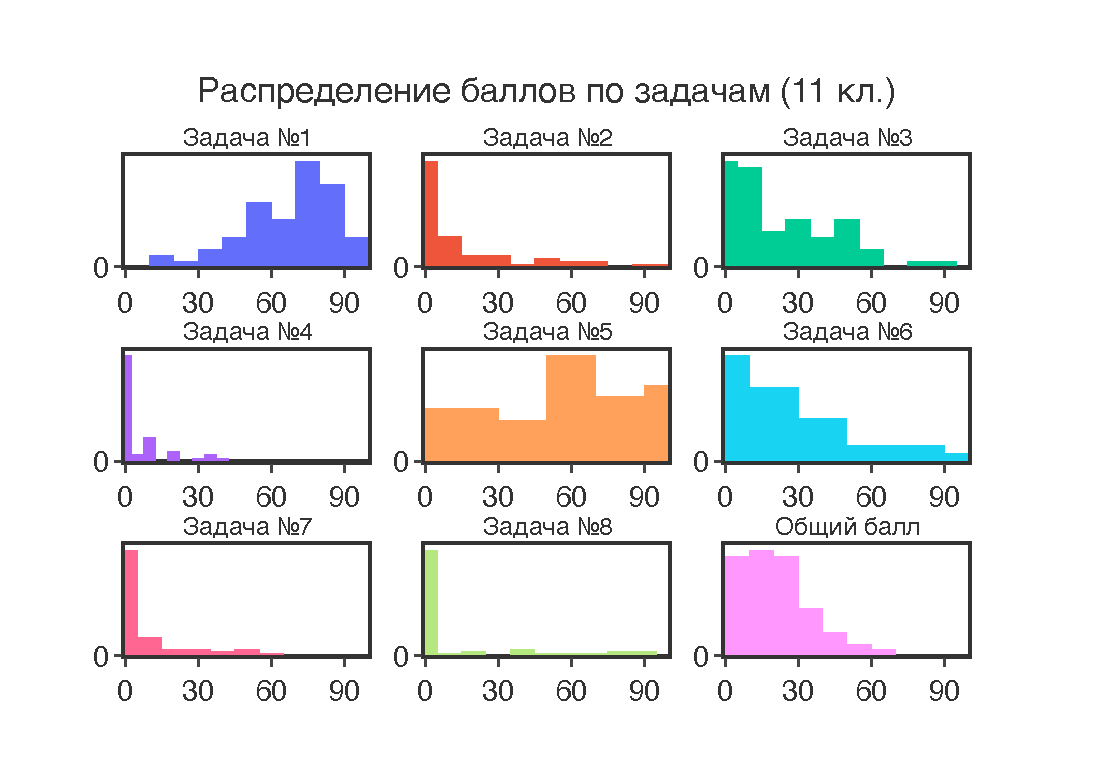
\includegraphics[width=\linewidth]{../export/pdf/results/2022/respa/grade11-dist-problemwise.pdf}


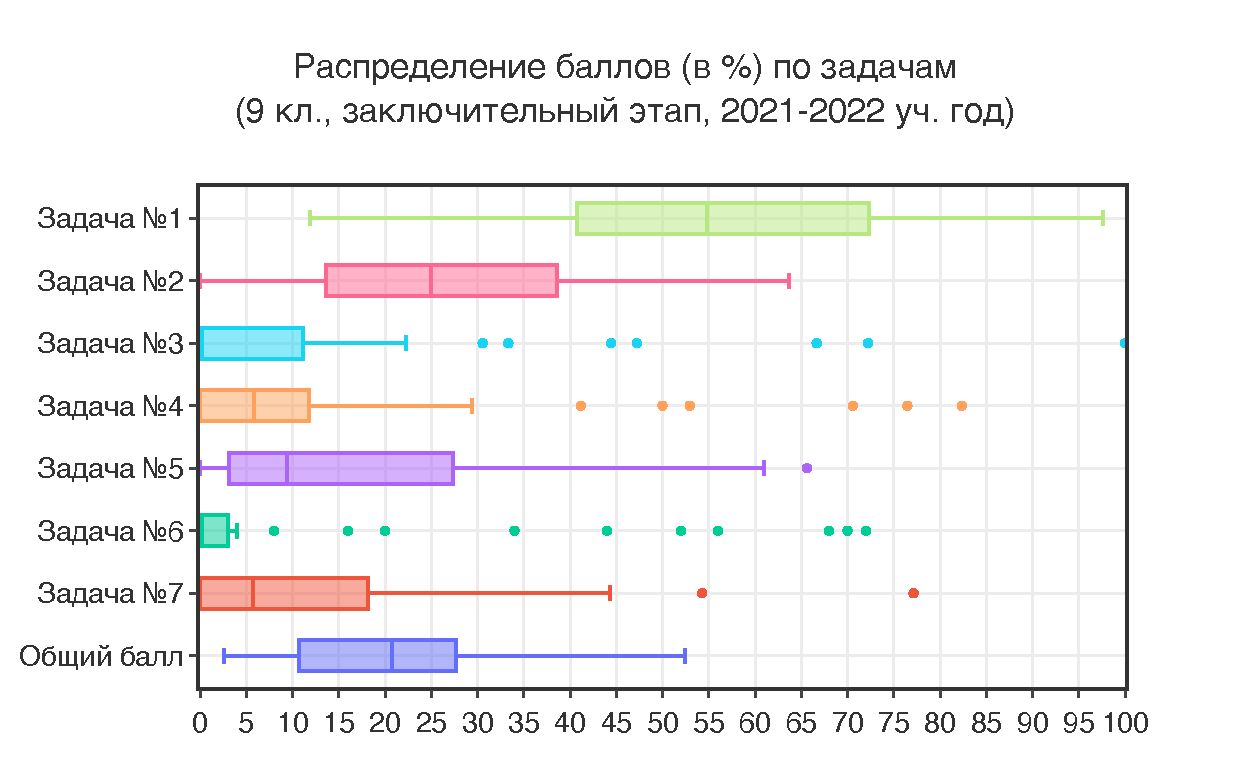
\includegraphics[width=\linewidth]{../export/pdf/results/2022/respa/grade9-dist-box.pdf}
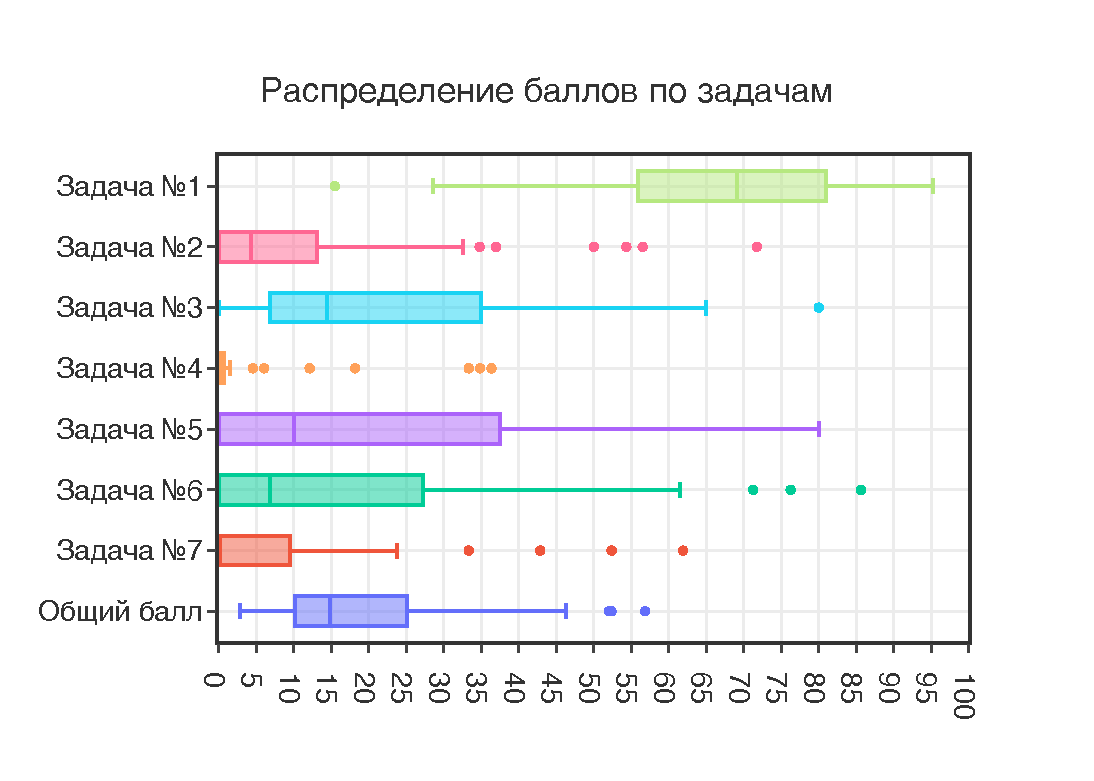
\includegraphics[width=\linewidth]{../export/pdf/results/2022/respa/grade10-dist-box.pdf}
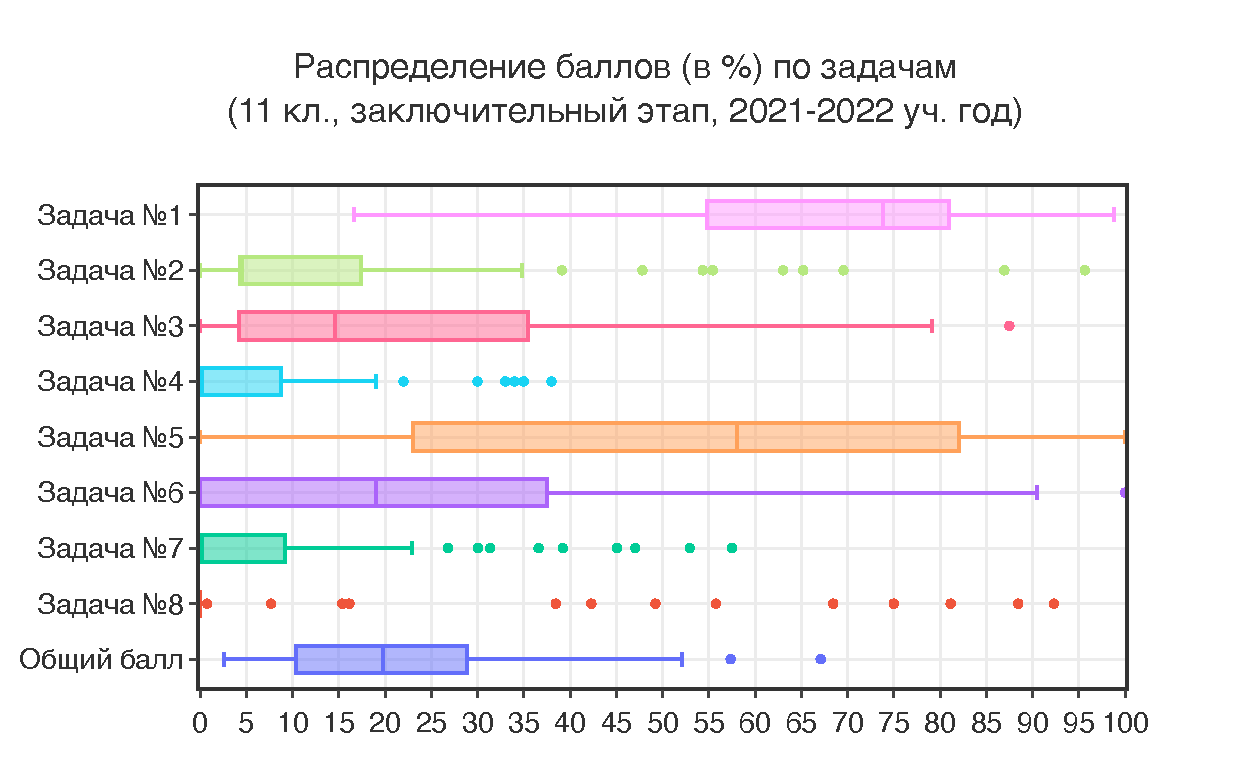
\includegraphics[width=\linewidth]{../export/pdf/results/2022/respa/grade11-dist-box.pdf}

\subsubsection{Результаты 2020-2021 уч. года}

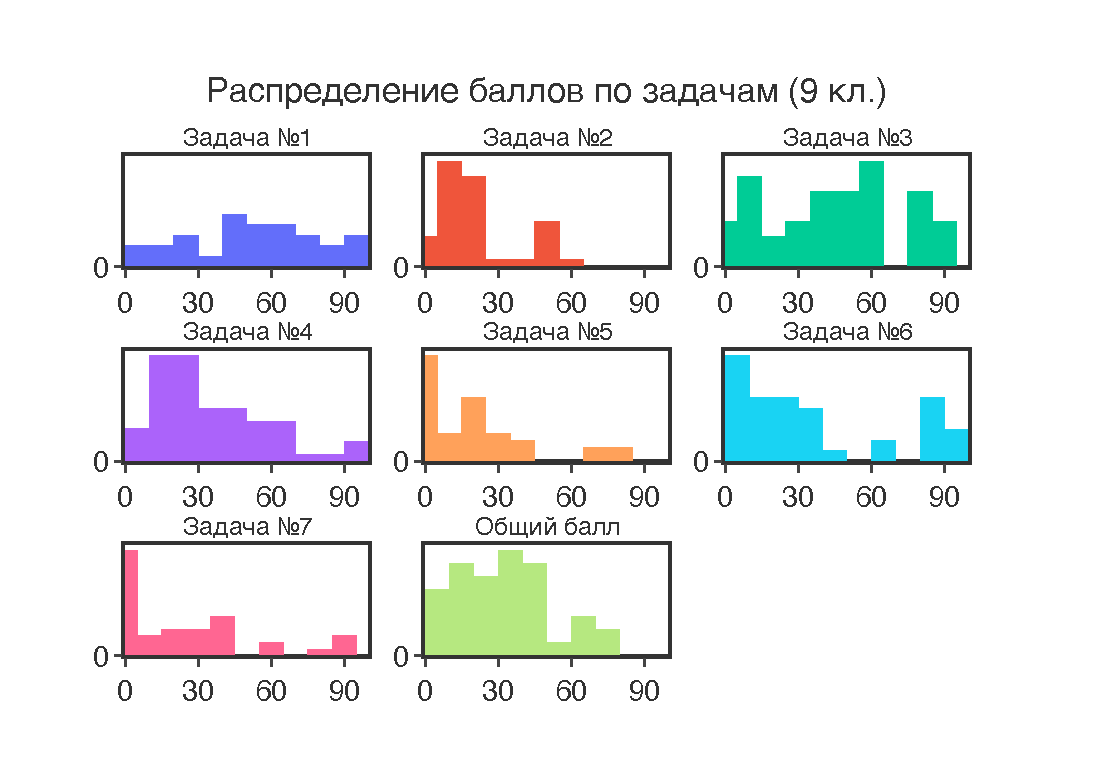
\includegraphics[width=\linewidth]{../export/pdf/results/2021/respa/grade9-dist-problemwise.pdf}
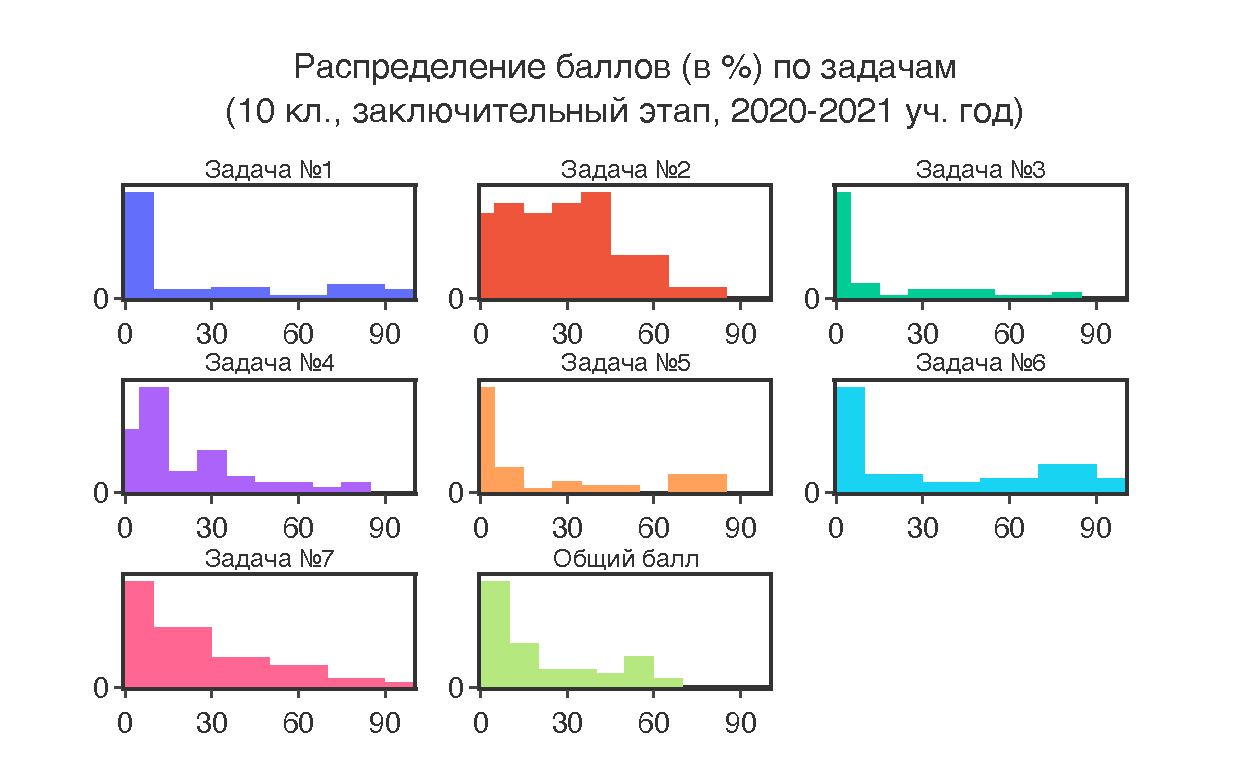
\includegraphics[width=\linewidth]{../export/pdf/results/2021/respa/grade10-dist-problemwise.pdf}
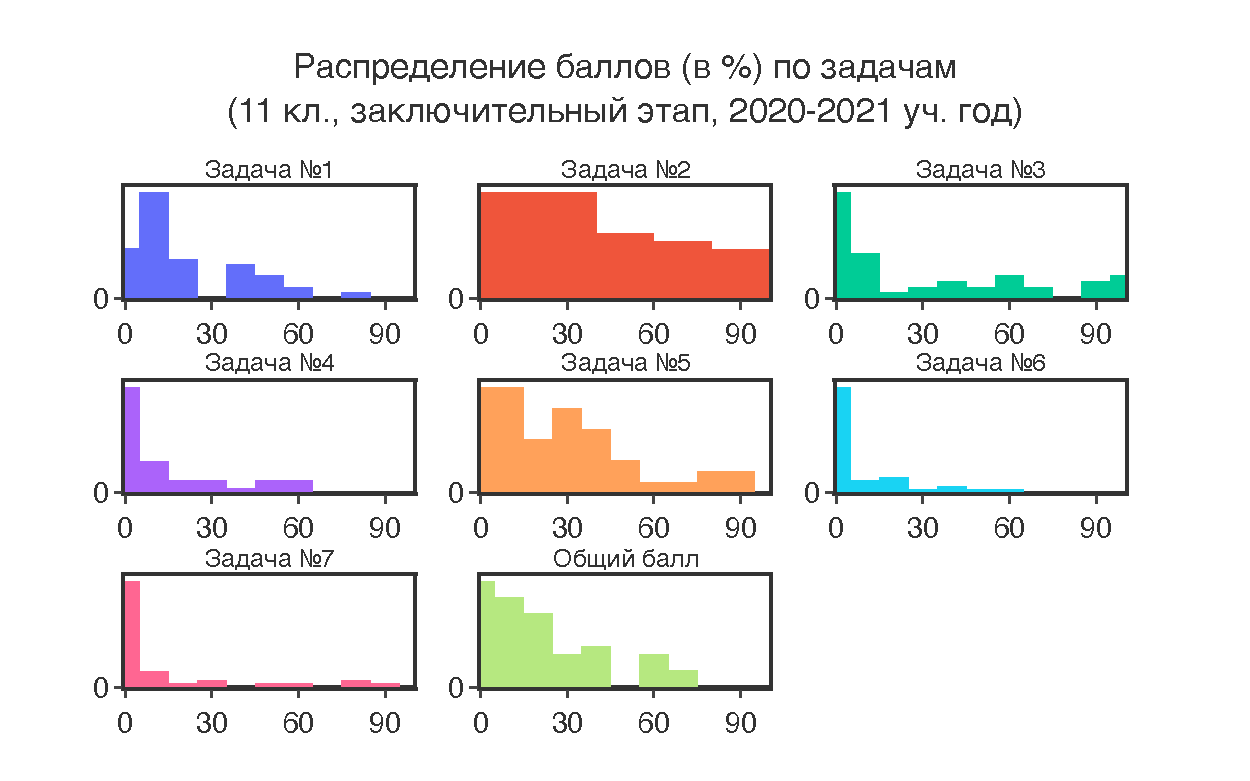
\includegraphics[width=\linewidth]{../export/pdf/results/2021/respa/grade11-dist-problemwise.pdf}


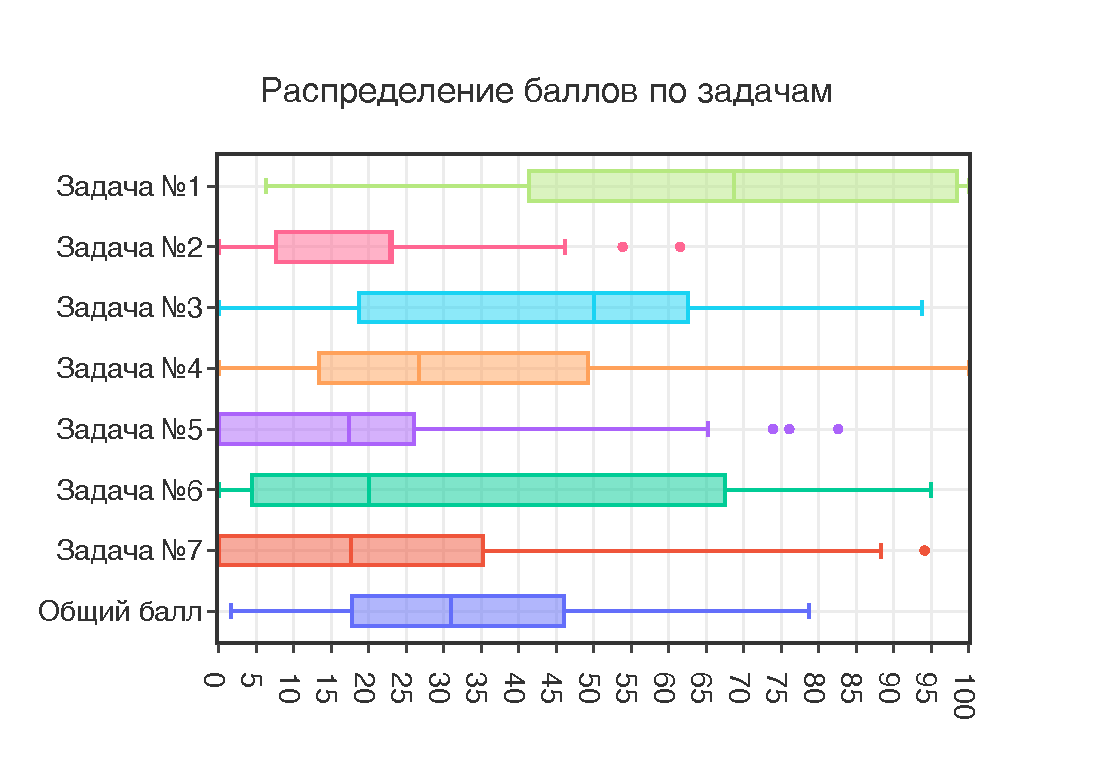
\includegraphics[width=\linewidth]{../export/pdf/results/2021/respa/grade9-dist-box.pdf}
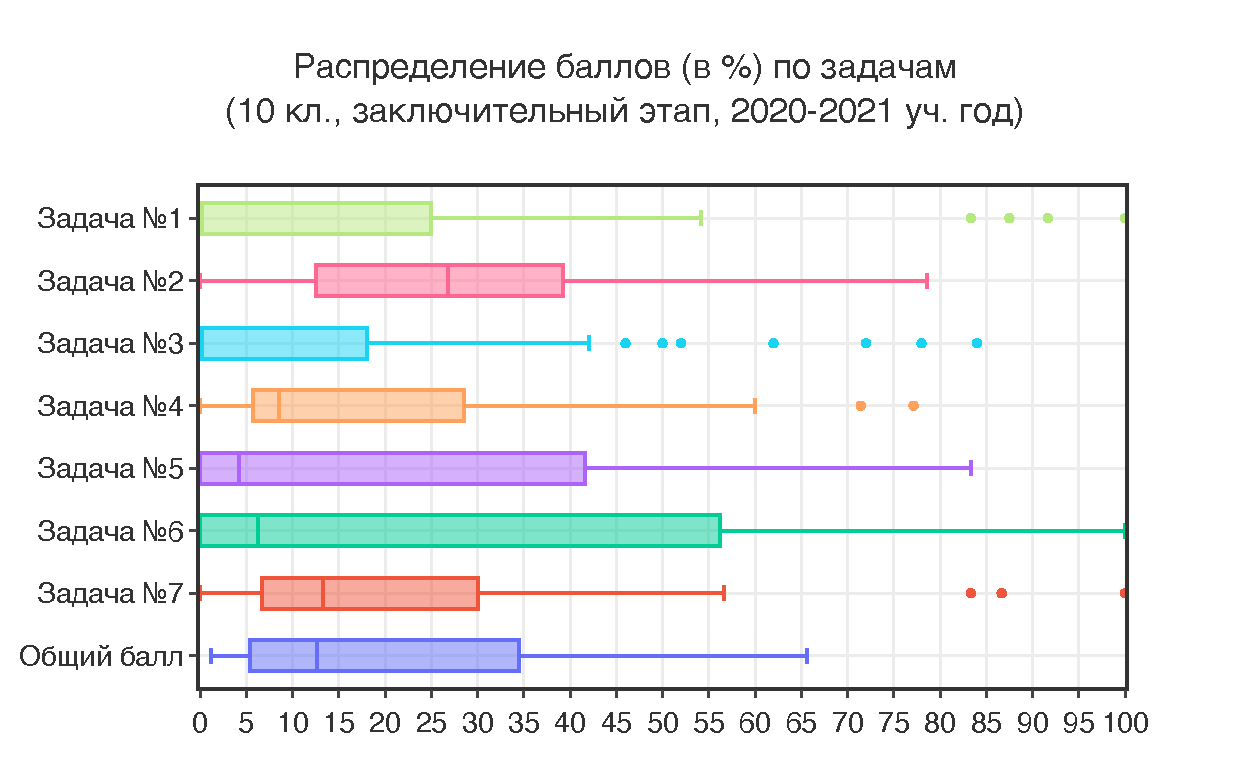
\includegraphics[width=\linewidth]{../export/pdf/results/2021/respa/grade10-dist-box.pdf}
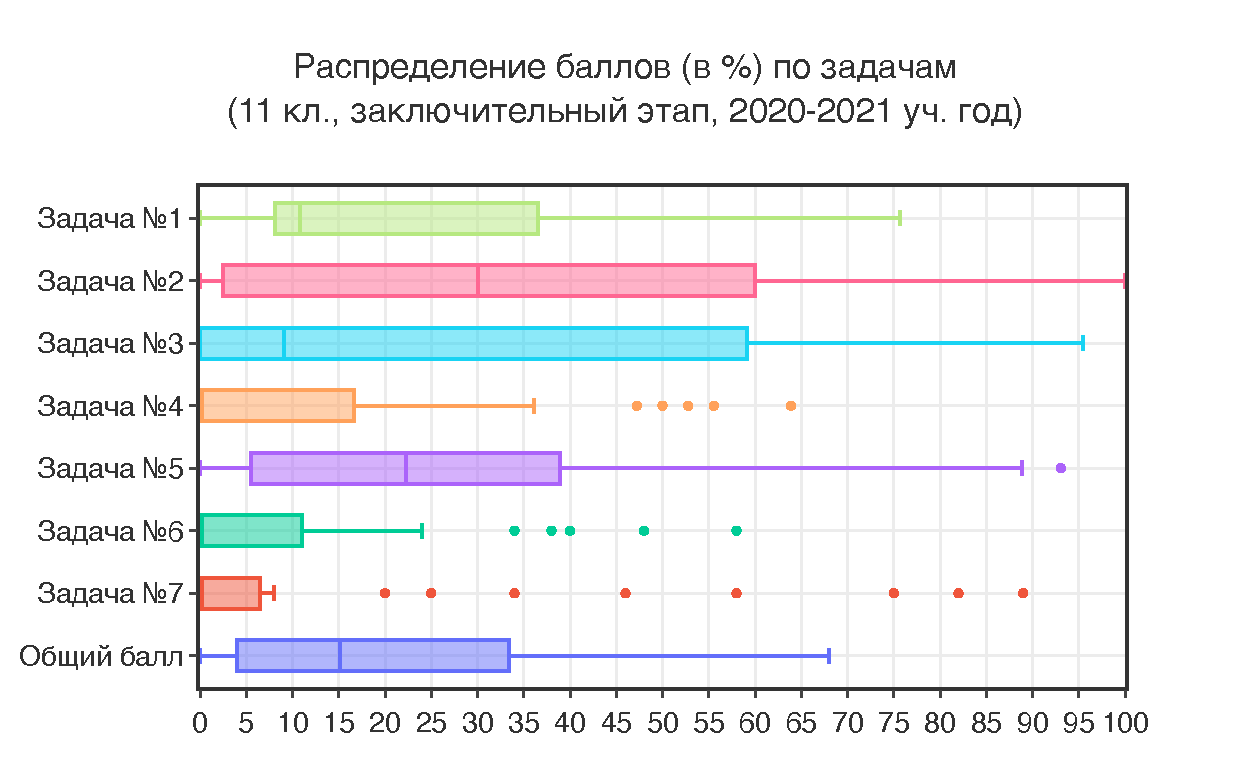
\includegraphics[width=\linewidth]{../export/pdf/results/2021/respa/grade11-dist-box.pdf}

\section{Корреляция областного и заключительного этапов}
Нас может интересовать - насколько результаты областного этапа коррелируют с результатами заключительного этапа? Иными словами, насколько хорошо выступление ученика на областном этапе (его баллы), предсказывают баллы этого ученика на заключительном этапе? Оценить корреляцию можно посчитав \href{https://en.wikipedia.org/wiki/Pearson_correlation_coefficient}{коэффициент Пирсона}. Коэффициент Пирсона $\rho$ - нормализованная ковариация двух массивов данных, принимает значение $\rho \in [-1, 1]$. Чем больше $|\rho|$, тем сильнее корреляция. Отрицательные значения $\rho$ показывают обратную корреляцию (например, чем больше баллов на областном этапе, тем меньше баллов на заключительном этапе). Коэффициенты Пирсона для баллов областного и заключительного этапов в 2022-2023 уч. году:

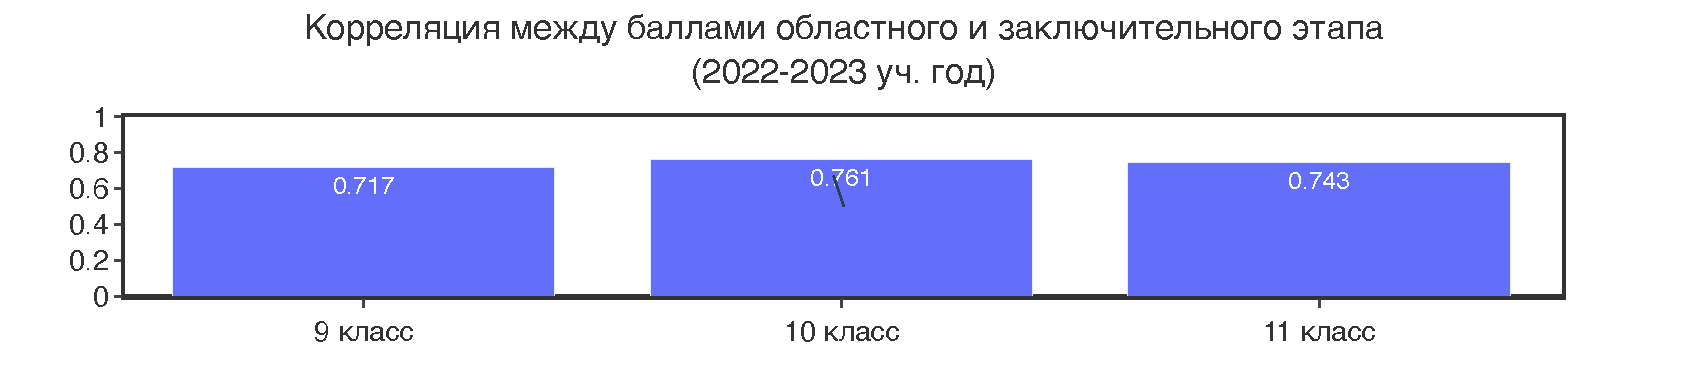
\includegraphics[width=\linewidth]{../export/pdf/trajectory/bygrade.pdf}

Посмотрим как выглядит зависимость графически:

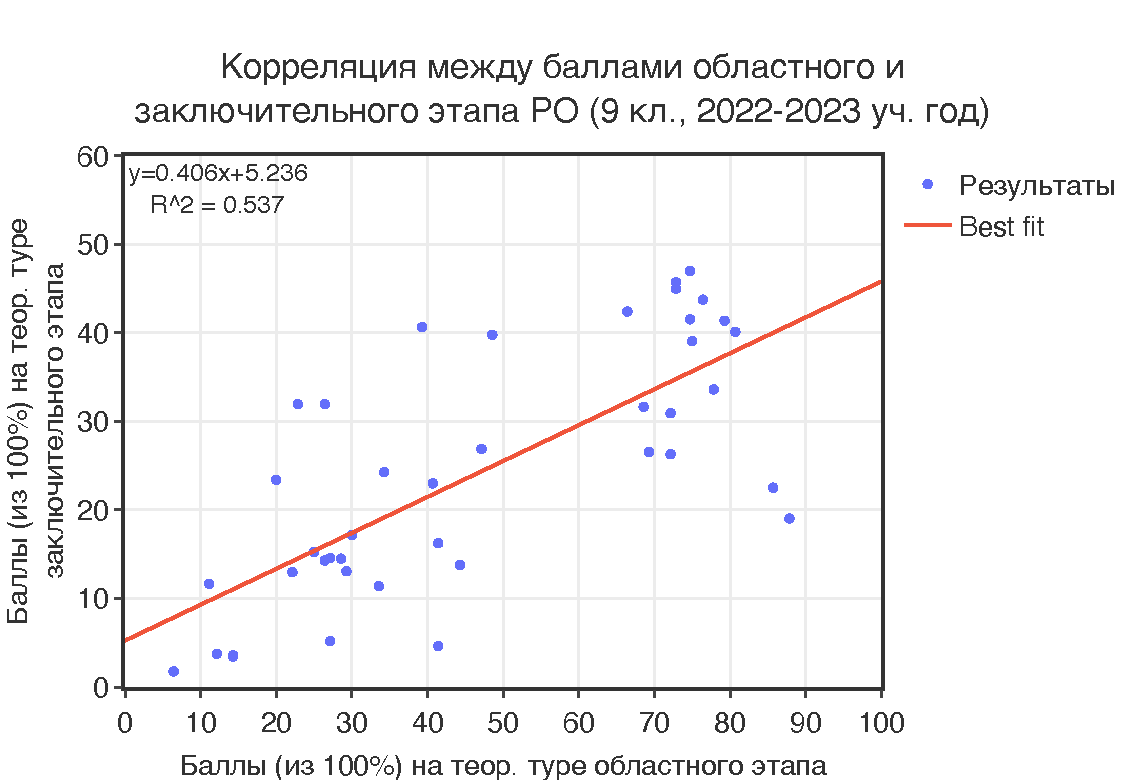
\includegraphics[width=\linewidth]{../export/pdf/trajectory/gr9-data.pdf}
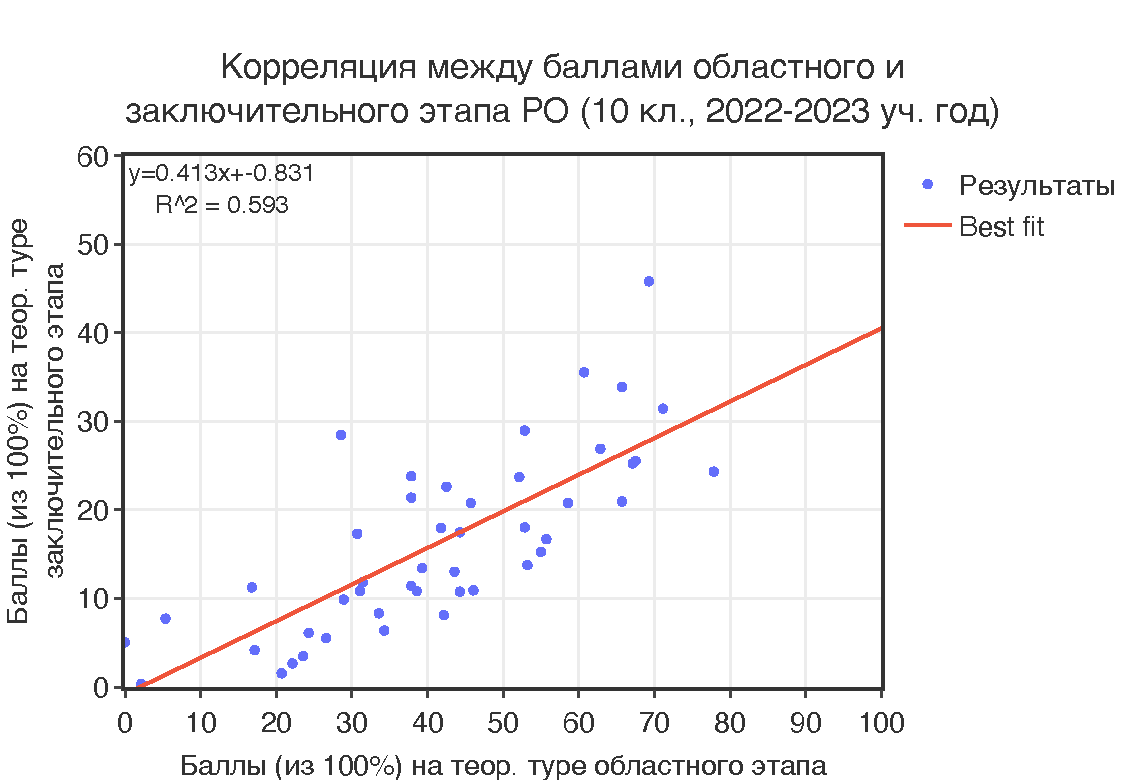
\includegraphics[width=\linewidth]{../export/pdf/trajectory/gr10-data.pdf}
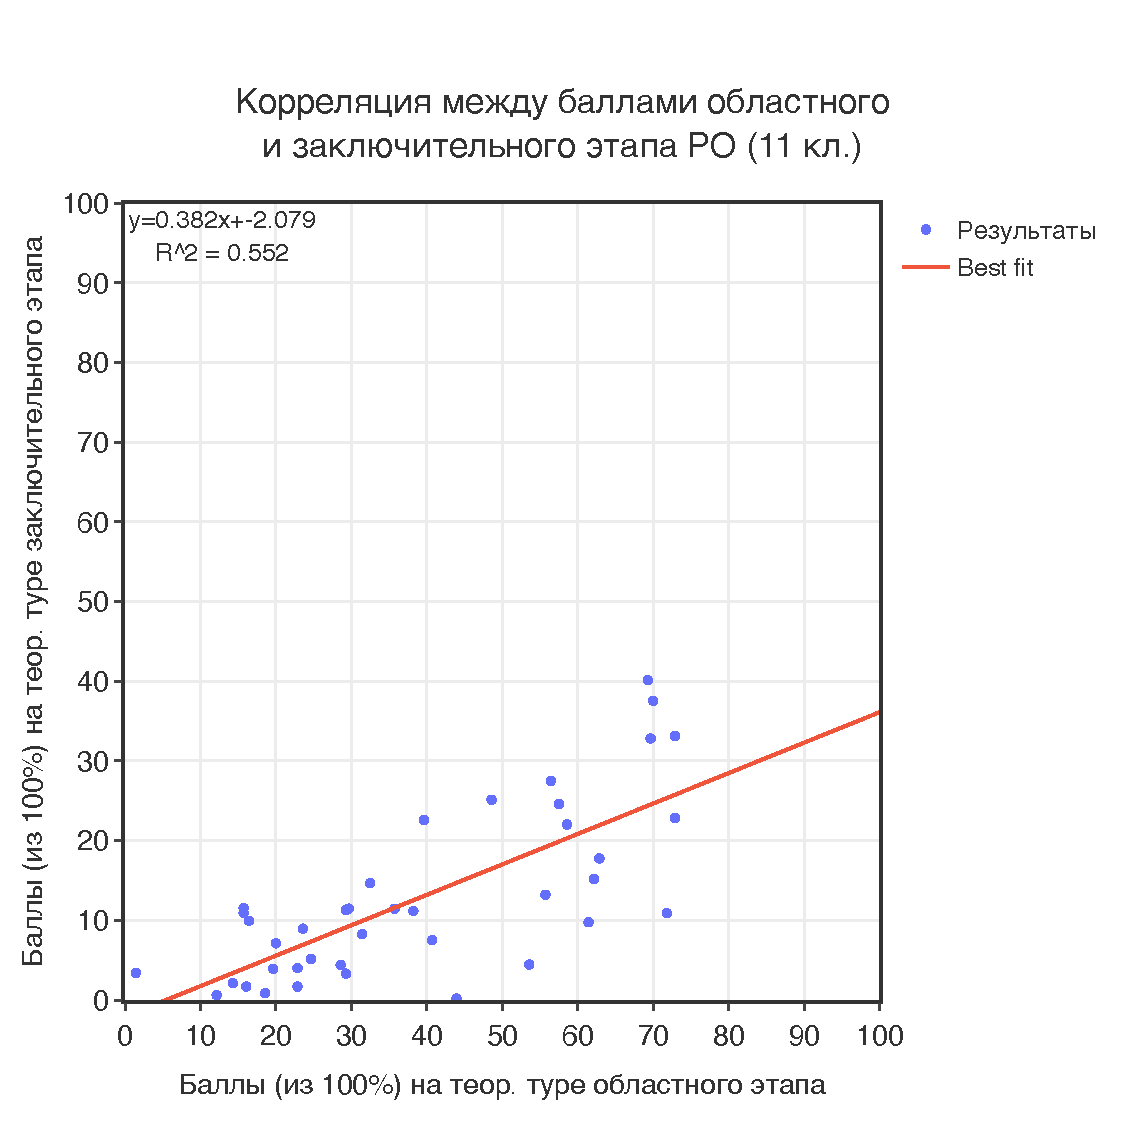
\includegraphics[width=\linewidth]{../export/pdf/trajectory/gr11-data.pdf}

Интересно было бы посмотреть как выглядит эта зависимость в разрезе областей. Поскольку с каждой области и каждого класса на заключительный этап проходит 2-3 человека, считать корреляцию для каждого класса по-отдельности не имеет смысла. Поэтому посчитаем корреляцию для трех классов сразу:

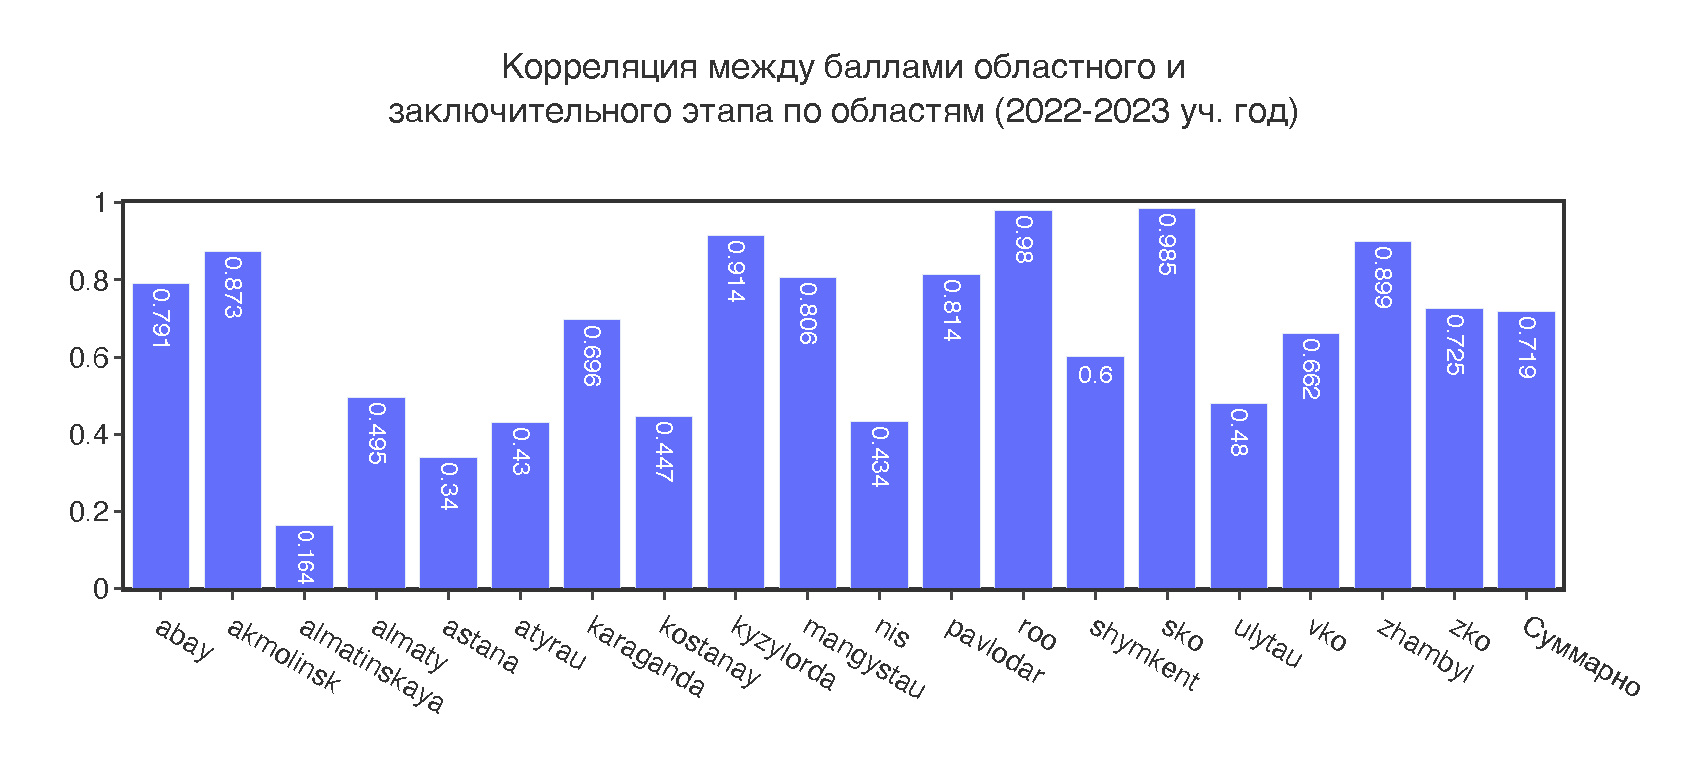
\includegraphics[width=\linewidth]{../export/pdf/trajectory/byoblast.pdf}

Вариация коэффициентов Пирсона поражает. Посмотрим как выглядит зависимость на примере некоторых областей (графики для всех областей есть \href{https://github.com/anmorgunov/respa-data-analysis/tree/main/export/pdf/trajectory}{в публичном репозитории на github}):

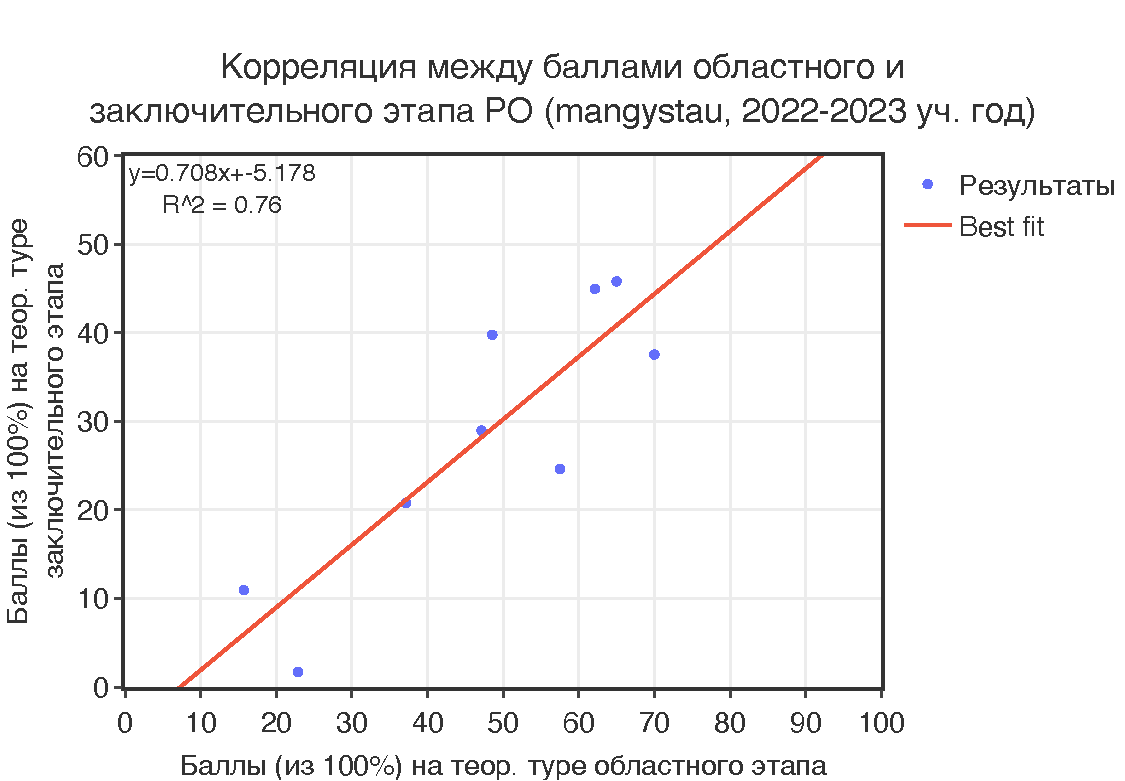
\includegraphics[width=\linewidth]{../export/pdf/trajectory/obl-mangystau.pdf}
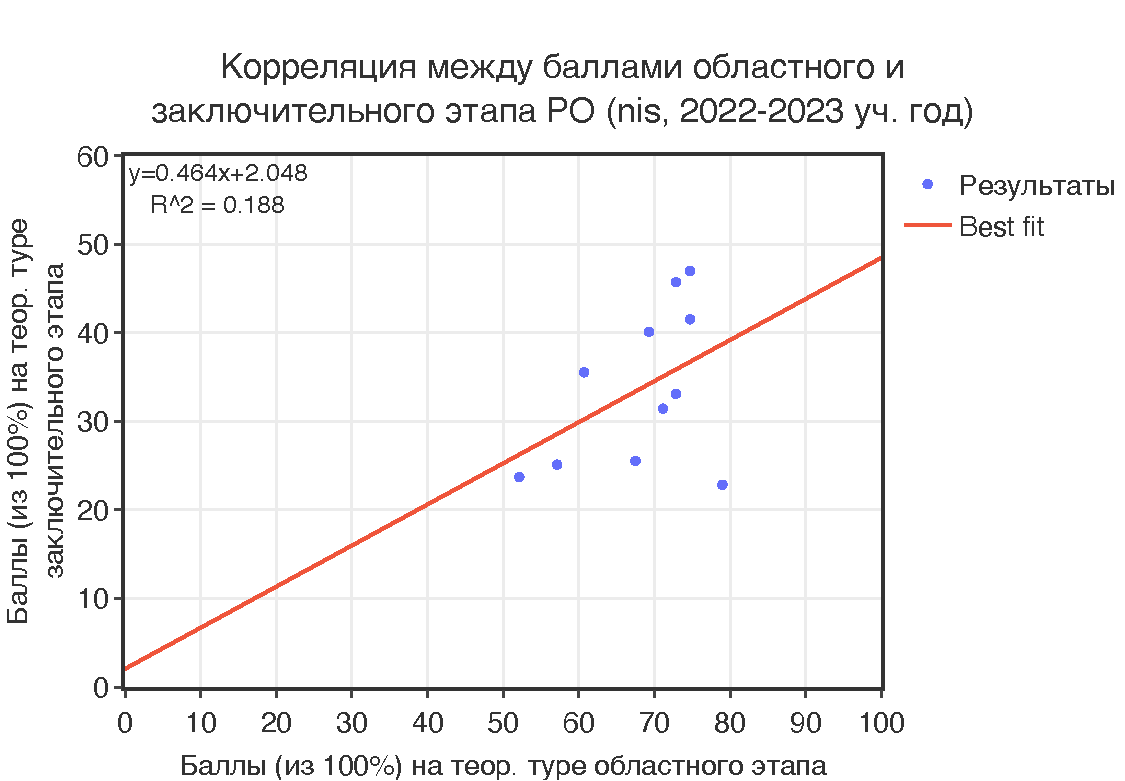
\includegraphics[width=\linewidth]{../export/pdf/trajectory/obl-nis.pdf}
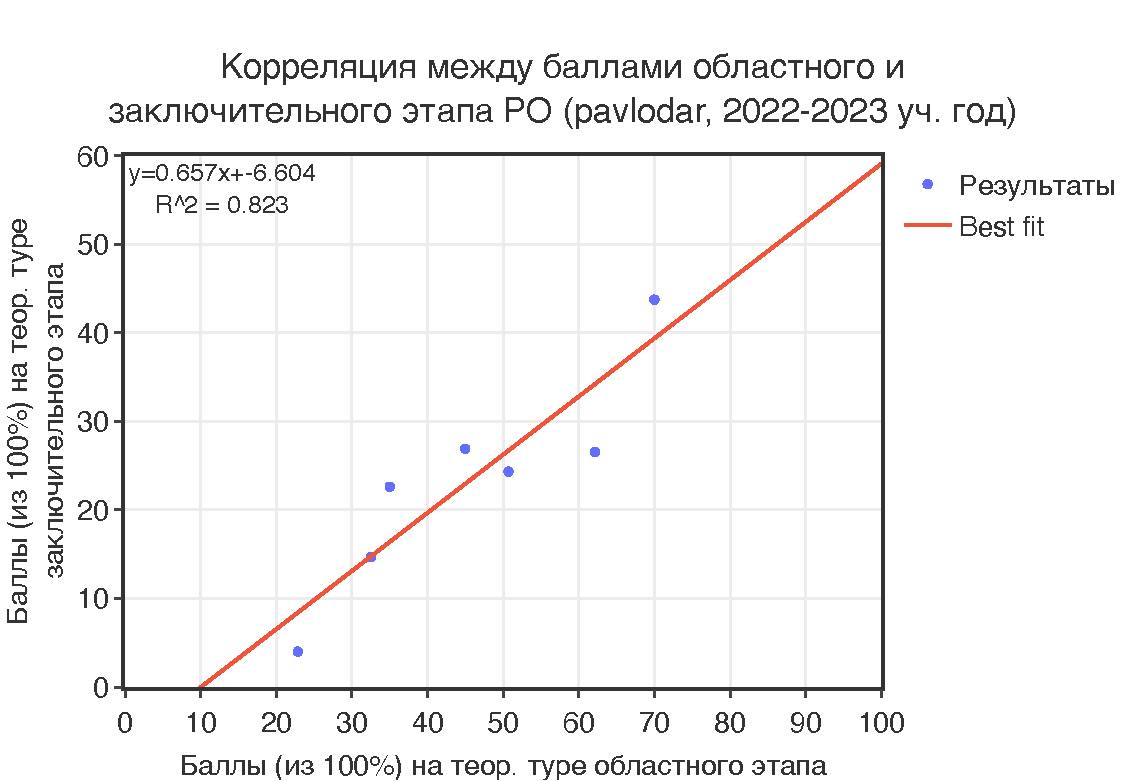
\includegraphics[width=\linewidth]{../export/pdf/trajectory/obl-pavlodar.pdf}

\section{Корреляция внутри комплекта заданий}

\subsection{Заключительный этап. 2022-2023.}

А что если посчитать коэффициенты Пирсона внутри одной олимпиады, для баллов за любые две задачи? Большой коэффициент Пирсона (напомним, значения коэффициента находятся в диапазоне от -1 до +1) означает, что если ученик набрал высокий балл по одной задаче, то скорее всего он набрал высокий балл и по другой задаче. С одной стороны, высокую корреляцию можно считать показателем сбалансированности комплекта с точки зрения сложности заданий. С другой стороны, сложно ожидать высокую корреляцию между баллами за задачу, скажем, по неорганической химии и органической химии. 

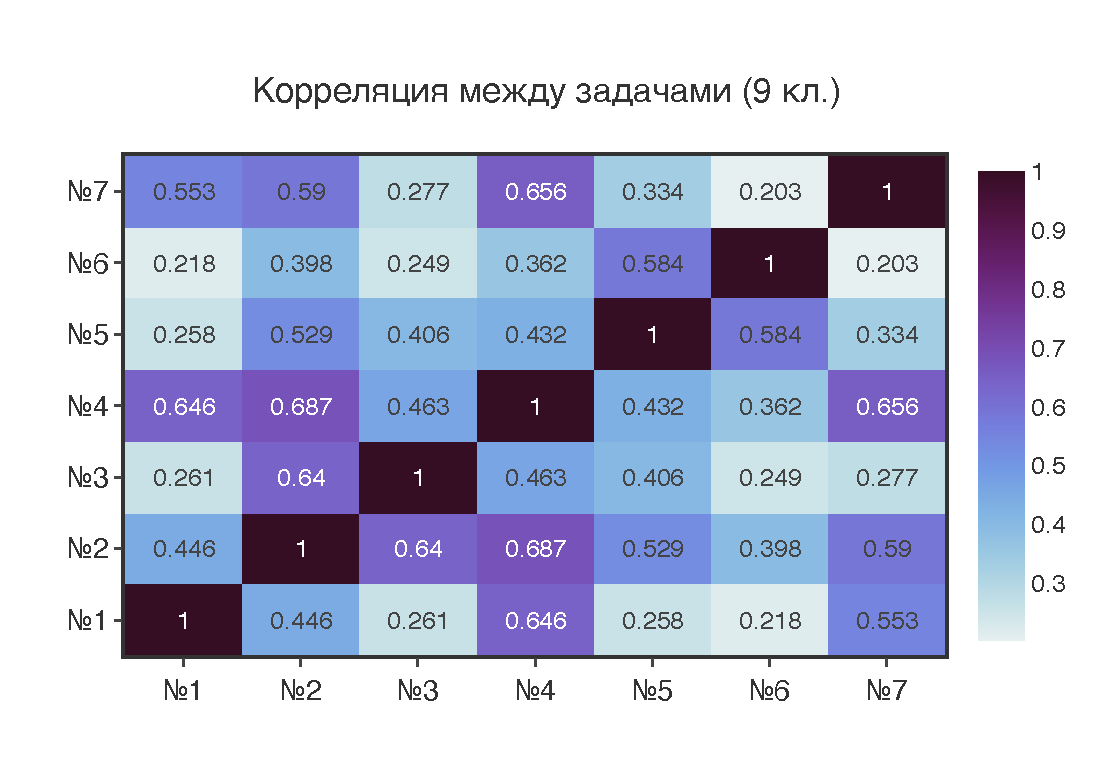
\includegraphics[width=\linewidth]{../export/pdf/results/2023/respa/grade9.pdf}

\newpage

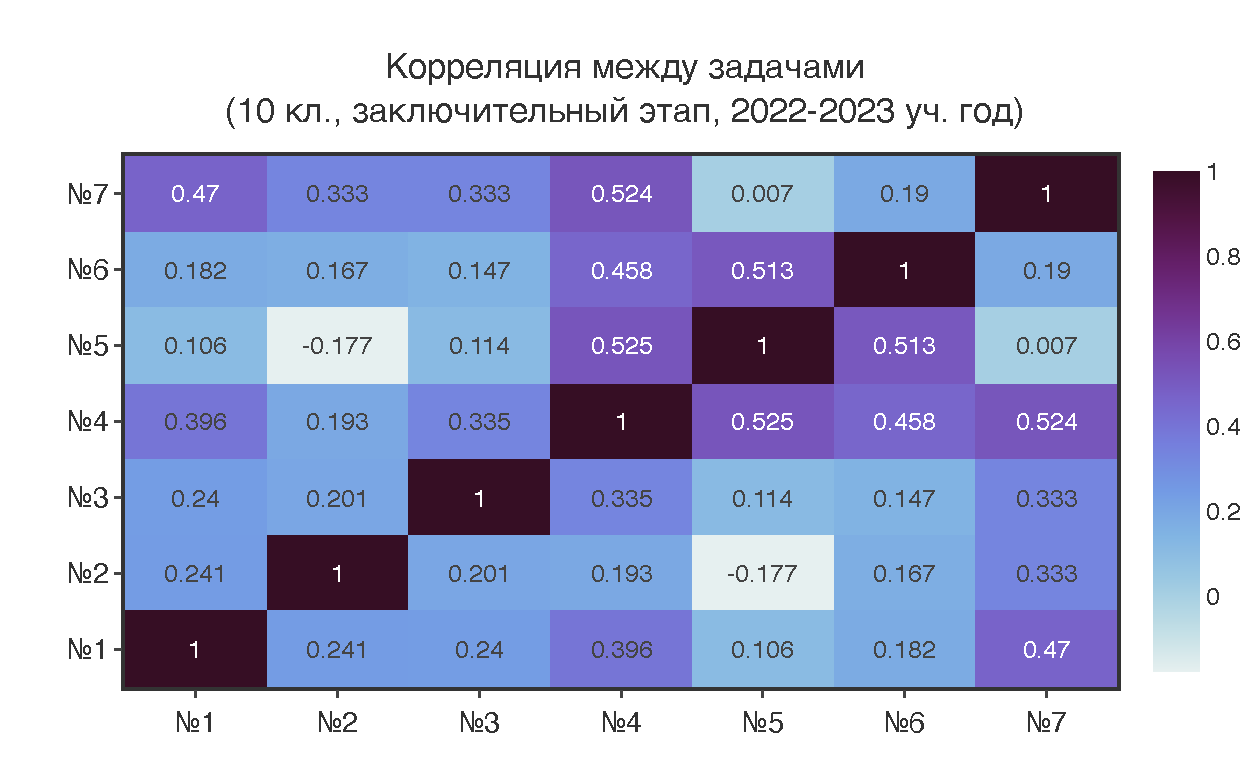
\includegraphics[width=\linewidth]{../export/pdf/results/2023/respa/grade10.pdf}

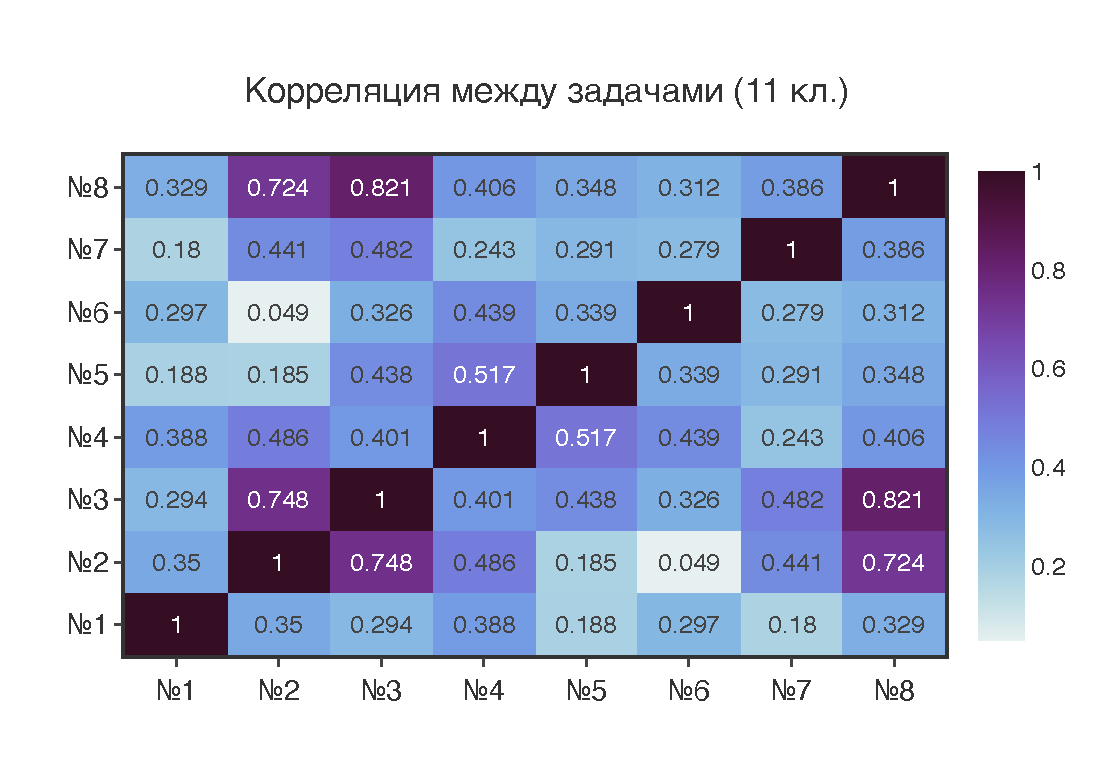
\includegraphics[width=\linewidth]{../export/pdf/results/2023/respa/grade11.pdf}

\newpage 

А что если мы попробуем посмотреть насколько одна-две любые задачи отличаются от остальных? Возьмем задачу $x$ и задачу $y$, посчитаем средний балл для каждого ученика и сравним со средними баллами за все задачи, кроме задач $x$ и $y$. Полученный коэффициент Пирсона отразим в ячейке $(x,y)$.

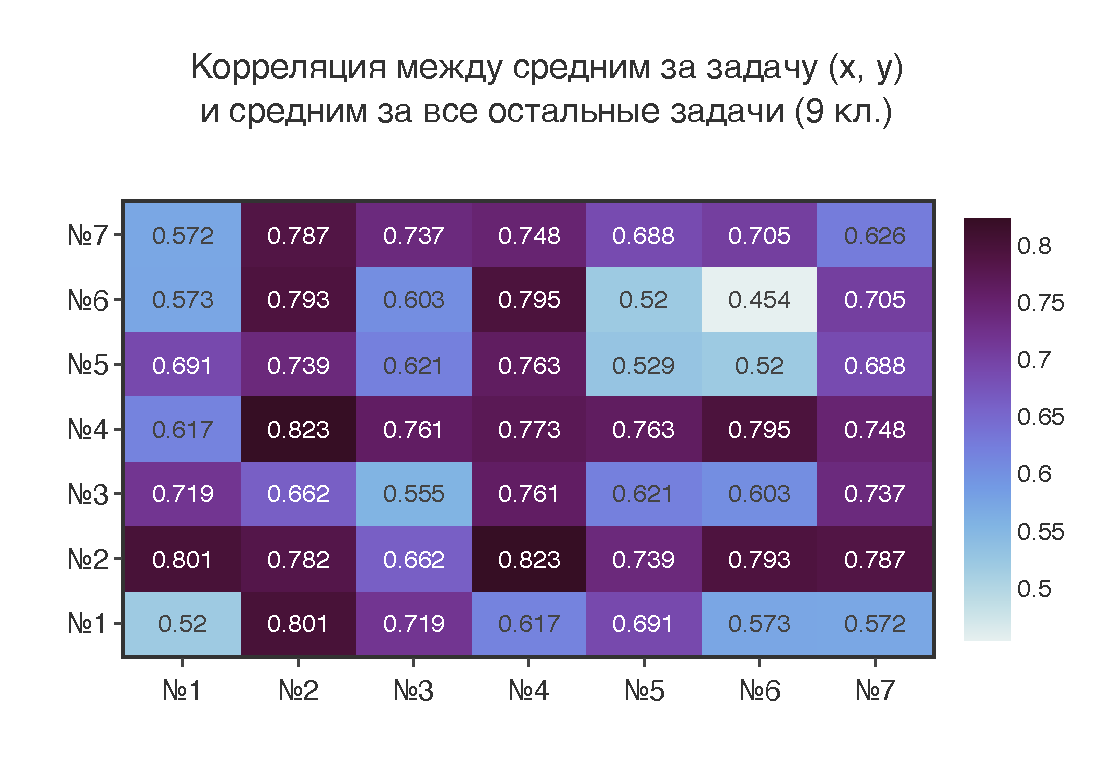
\includegraphics[width=\linewidth]{../export/pdf/results/2023/respa/grade9-avg.pdf}

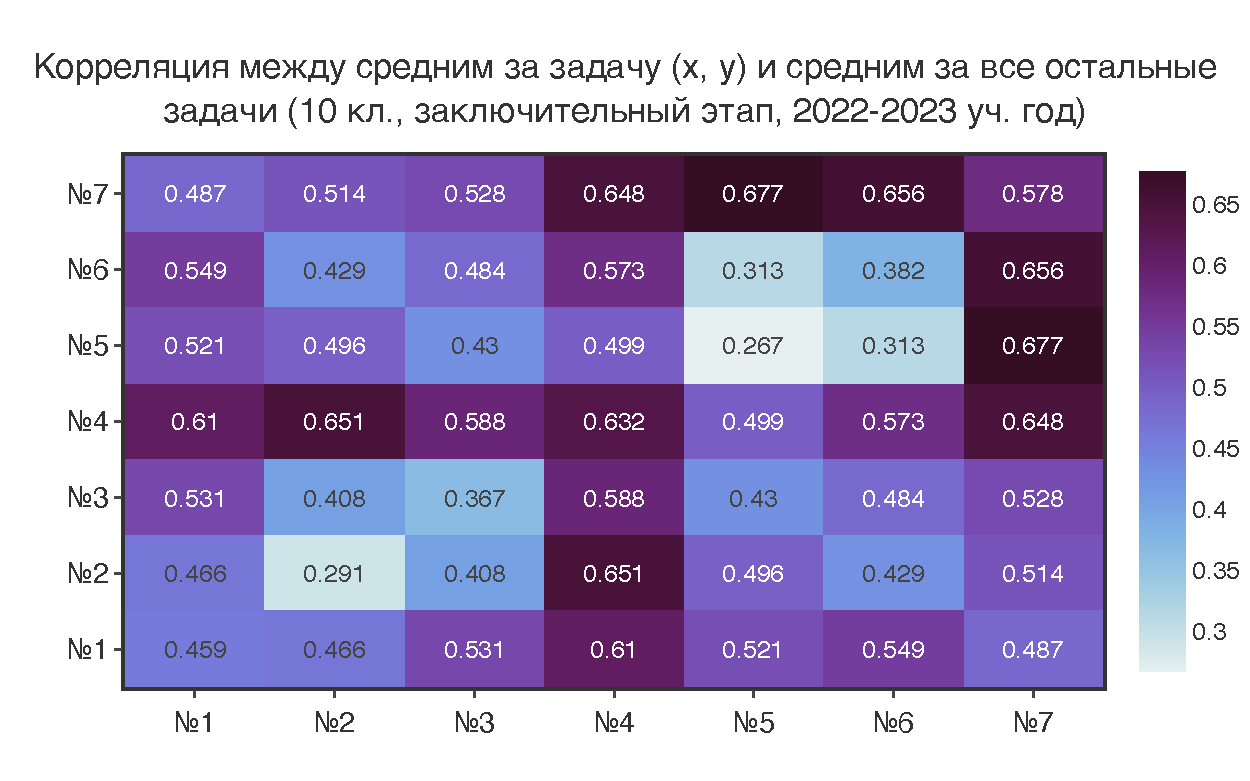
\includegraphics[width=\linewidth]{../export/pdf/results/2023/respa/grade10-avg.pdf}

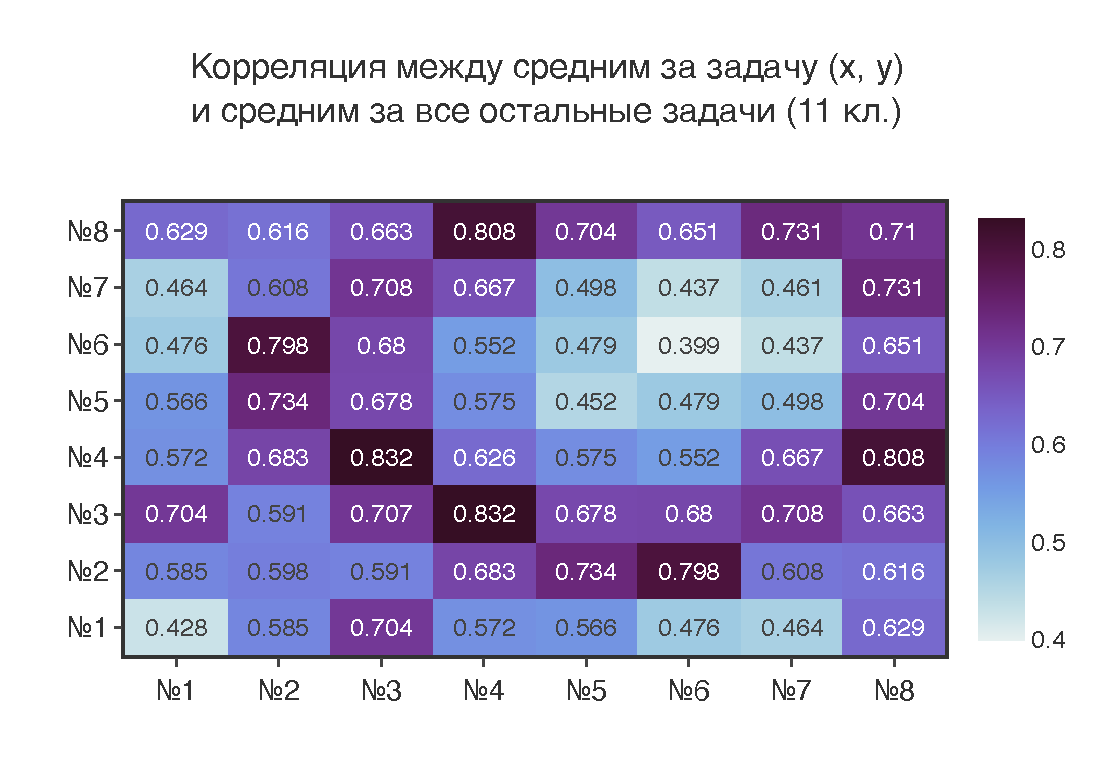
\includegraphics[width=\linewidth]{../export/pdf/results/2023/respa/grade11-avg.pdf}

\subsection{Областной этап. 2022-2023.}
Повторим те же расчеты для заданий областного этапа.

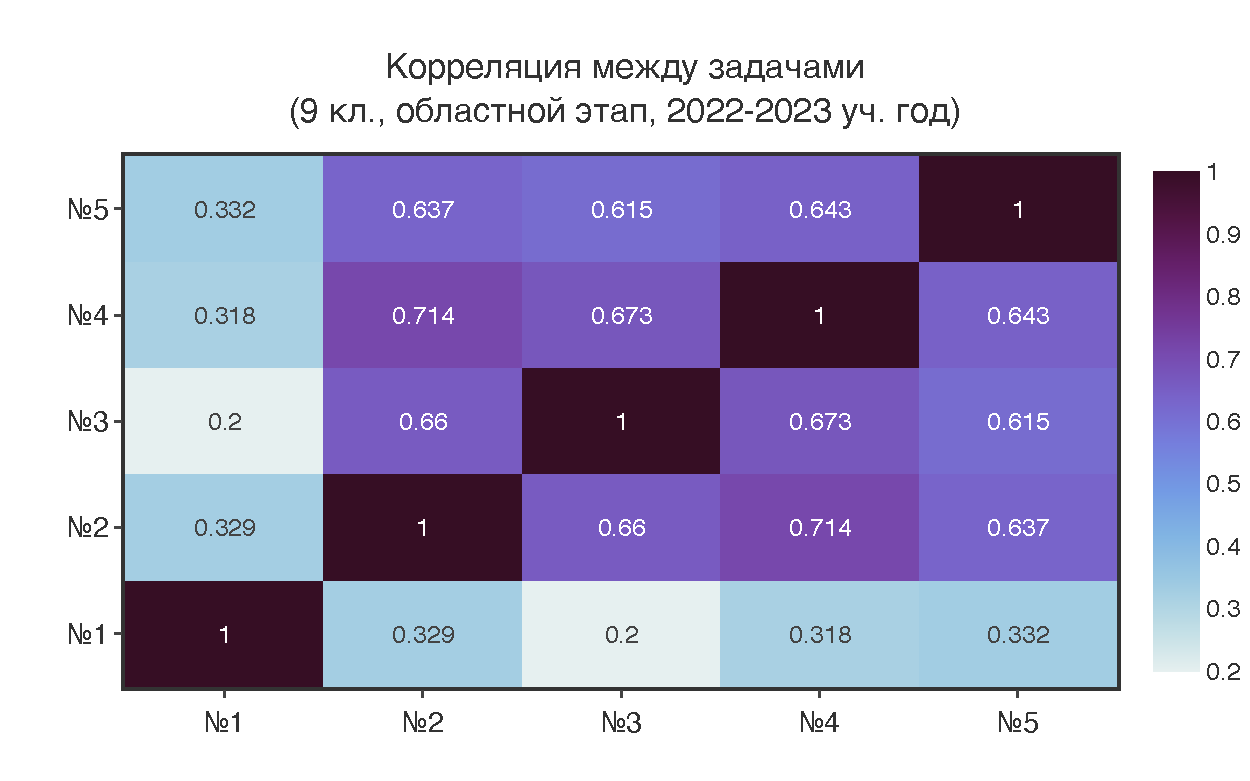
\includegraphics[width=\linewidth]{../export/pdf/results/2023/oblast/grade9.pdf}

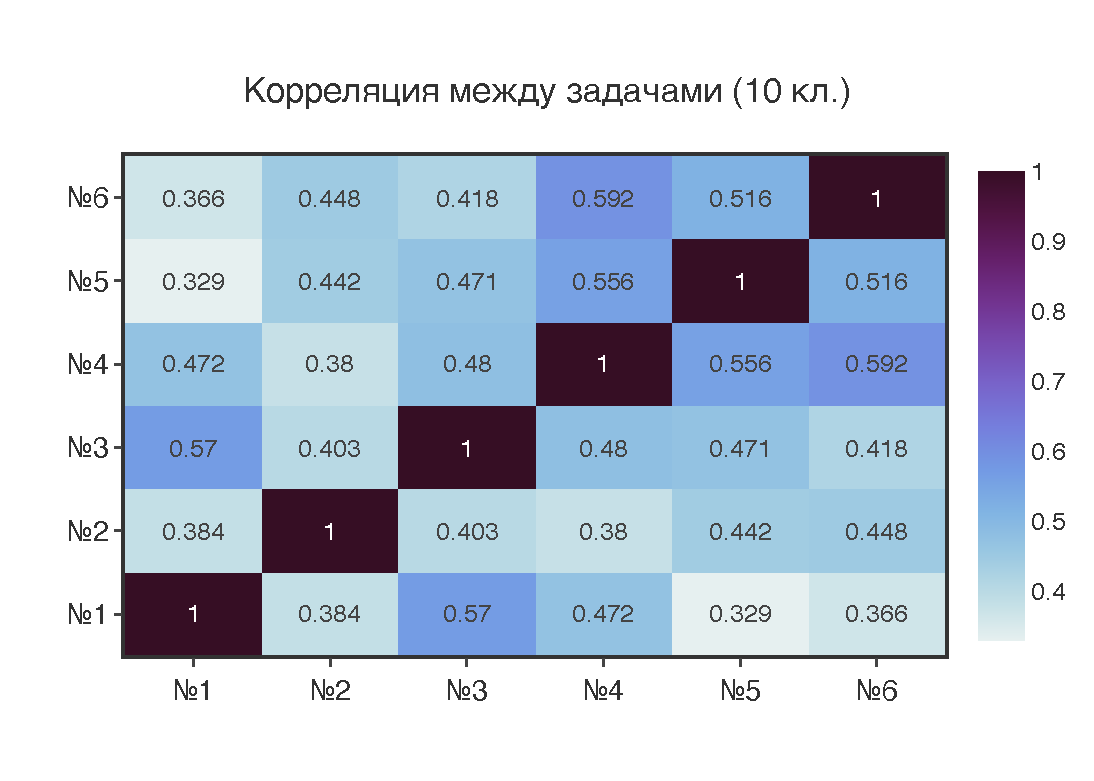
\includegraphics[width=\linewidth]{../export/pdf/results/2023/oblast/grade10.pdf}

\includegraphics[width=\linewidth]{../export/pdf/results/2023/oblast/grade11.pdf}

\includegraphics[width=\linewidth]{../export/pdf/results/2023/oblast/grade9-avg.pdf}

\includegraphics[width=\linewidth]{../export/pdf/results/2023/oblast/grade10-avg.pdf}

\includegraphics[width=\linewidth]{../export/pdf/results/2023/oblast/grade11-avg.pdf}

\subsection{Заключительный этап. 2021-2022.}

Для сравнения, повторим те же расчеты для заключительного этапа 2021-2022 уч. года.

\includegraphics[width=\linewidth]{../export/pdf/results/2022/respa/grade9.pdf}

\includegraphics[width=\linewidth]{../export/pdf/results/2022/respa/grade10.pdf}

\includegraphics[width=\linewidth]{../export/pdf/results/2022/respa/grade11.pdf}

\includegraphics[width=\linewidth]{../export/pdf/results/2022/respa/grade9-avg.pdf}

\includegraphics[width=\linewidth]{../export/pdf/results/2022/respa/grade10-avg.pdf}

\includegraphics[width=\linewidth]{../export/pdf/results/2022/respa/grade11-avg.pdf}

\subsection{Заключительный этап. 2020-2021.}

Для сравнения, повторим те же расчеты для заключительного этапа 2020-2021 уч. года.

\includegraphics[width=\linewidth]{../export/pdf/results/2021/respa/grade9.pdf}

\includegraphics[width=\linewidth]{../export/pdf/results/2021/respa/grade10.pdf}

\includegraphics[width=\linewidth]{../export/pdf/results/2021/respa/grade11.pdf}

\includegraphics[width=\linewidth]{../export/pdf/results/2021/respa/grade9-avg.pdf}

\includegraphics[width=\linewidth]{../export/pdf/results/2021/respa/grade10-avg.pdf}

\includegraphics[width=\linewidth]{../export/pdf/results/2021/respa/grade11-avg.pdf}

\newpage 

\section{Способность учеников к самостоятельной оценке}

В рамках онлайн-опросов, проводившихся в текущем учебном году, ученикам предлагалось оценить насколько хорошо они решили ту или иную задачу выбрав один из четырех вариантов ответов:

\begin{itemize}
    \itemsep-0.3em
    \item[--] Я не решил(а) эту задачу и я даже не знал(а) с чего начать
    \item[--] У меня были идеи по решению задачи, но я не смог(ла) их довести до ума
    \item[--] Я решил(а) задачу, но думаю у меня есть ошибки
    \item[--] Я решил(а) эту задачу и уверен, что решил(а) правильно на 80\% и больше.
\end{itemize}

Нам стало интересно: а насколько эта самооценка коррелирует с истинным результатом? Cначала посмотрим на все классы вместе, а затем на каждый класс по отдельности. Графики для индивидуальных задач есть \href{https://github.com/anmorgunov/respa-data-analysis/tree/main/export/pdf/selfassessment/respa}{в публичном репозитории на github}.

\includegraphics[width=\linewidth]{../export/pdf/selfassessment/respa/allgrade-box.pdf}
\includegraphics[width=\linewidth]{../export/pdf/selfassessment/respa/grade9-box.pdf}
\includegraphics[width=\linewidth]{../export/pdf/selfassessment/respa/grade10-box.pdf}
\includegraphics[width=\linewidth]{../export/pdf/selfassessment/respa/grade11-box.pdf}

Повторим тоже самое для областного этапа:

\includegraphics[width=\linewidth]{../export/pdf/selfassessment/oblast/allgrade-box.pdf}
\includegraphics[width=\linewidth]{../export/pdf/selfassessment/oblast/grade9-box.pdf}
\includegraphics[width=\linewidth]{../export/pdf/selfassessment/oblast/grade10-box.pdf}
\includegraphics[width=\linewidth]{../export/pdf/selfassessment/oblast/grade11-box.pdf}



\end{document}
